\PassOptionsToPackage{unicode=true}{hyperref} % options for packages loaded elsewhere
\PassOptionsToPackage{hyphens}{url}
%
\documentclass[8pt,ignorenonframetext,aspectratio=169]{beamer}
\usepackage{pgfpages}
\setbeamertemplate{caption}[numbered]
\setbeamertemplate{caption label separator}{: }
\setbeamercolor{caption name}{fg=normal text.fg}
\beamertemplatenavigationsymbolsempty
% Prevent slide breaks in the middle of a paragraph:
\widowpenalties 1 10000
\raggedbottom
\setbeamertemplate{part page}{
\centering
\begin{beamercolorbox}[sep=16pt,center]{part title}
  \usebeamerfont{part title}\insertpart\par
\end{beamercolorbox}
}
\setbeamertemplate{section page}{
\centering
\begin{beamercolorbox}[sep=12pt,center]{part title}
  \usebeamerfont{section title}\insertsection\par
\end{beamercolorbox}
}
\setbeamertemplate{subsection page}{
\centering
\begin{beamercolorbox}[sep=8pt,center]{part title}
  \usebeamerfont{subsection title}\insertsubsection\par
\end{beamercolorbox}
}
\AtBeginPart{
  \frame{\partpage}
}
\AtBeginSection{
  \ifbibliography
  \else
    \frame{\sectionpage}
  \fi
}
\AtBeginSubsection{
  \frame{\subsectionpage}
}
\usepackage{lmodern}
\usepackage{amssymb,amsmath}
\usepackage{ifxetex,ifluatex}
\usepackage{fixltx2e} % provides \textsubscript
\ifnum 0\ifxetex 1\fi\ifluatex 1\fi=0 % if pdftex
  \usepackage[T1]{fontenc}
  \usepackage[utf8]{inputenc}
  \usepackage{textcomp} % provides euro and other symbols
\else % if luatex or xelatex
  \usepackage{unicode-math}
  \defaultfontfeatures{Ligatures=TeX,Scale=MatchLowercase}
\fi
% use upquote if available, for straight quotes in verbatim environments
\IfFileExists{upquote.sty}{\usepackage{upquote}}{}
% use microtype if available
\IfFileExists{microtype.sty}{%
\usepackage[]{microtype}
\UseMicrotypeSet[protrusion]{basicmath} % disable protrusion for tt fonts
}{}
\IfFileExists{parskip.sty}{%
\usepackage{parskip}
}{% else
\setlength{\parindent}{0pt}
\setlength{\parskip}{6pt plus 2pt minus 1pt}
}
\usepackage{hyperref}
\hypersetup{
            pdftitle={ NMdata: A fast R package for efficient data preparation, consistency-checking and post-processing in PK/PD modeling},
            pdfauthor={Philip Delff},
            pdfborder={0 0 0},
            breaklinks=true}
\urlstyle{same}  % don't use monospace font for urls
\newif\ifbibliography
\usepackage{color}
\usepackage{fancyvrb}
\newcommand{\VerbBar}{|}
\newcommand{\VERB}{\Verb[commandchars=\\\{\}]}
\DefineVerbatimEnvironment{Highlighting}{Verbatim}{commandchars=\\\{\}}
% Add ',fontsize=\small' for more characters per line
\usepackage{framed}
\definecolor{shadecolor}{RGB}{248,248,248}
\newenvironment{Shaded}{\begin{snugshade}}{\end{snugshade}}
\newcommand{\AlertTok}[1]{\textcolor[rgb]{0.94,0.16,0.16}{#1}}
\newcommand{\AnnotationTok}[1]{\textcolor[rgb]{0.56,0.35,0.01}{\textbf{\textit{#1}}}}
\newcommand{\AttributeTok}[1]{\textcolor[rgb]{0.77,0.63,0.00}{#1}}
\newcommand{\BaseNTok}[1]{\textcolor[rgb]{0.00,0.00,0.81}{#1}}
\newcommand{\BuiltInTok}[1]{#1}
\newcommand{\CharTok}[1]{\textcolor[rgb]{0.31,0.60,0.02}{#1}}
\newcommand{\CommentTok}[1]{\textcolor[rgb]{0.56,0.35,0.01}{\textit{#1}}}
\newcommand{\CommentVarTok}[1]{\textcolor[rgb]{0.56,0.35,0.01}{\textbf{\textit{#1}}}}
\newcommand{\ConstantTok}[1]{\textcolor[rgb]{0.00,0.00,0.00}{#1}}
\newcommand{\ControlFlowTok}[1]{\textcolor[rgb]{0.13,0.29,0.53}{\textbf{#1}}}
\newcommand{\DataTypeTok}[1]{\textcolor[rgb]{0.13,0.29,0.53}{#1}}
\newcommand{\DecValTok}[1]{\textcolor[rgb]{0.00,0.00,0.81}{#1}}
\newcommand{\DocumentationTok}[1]{\textcolor[rgb]{0.56,0.35,0.01}{\textbf{\textit{#1}}}}
\newcommand{\ErrorTok}[1]{\textcolor[rgb]{0.64,0.00,0.00}{\textbf{#1}}}
\newcommand{\ExtensionTok}[1]{#1}
\newcommand{\FloatTok}[1]{\textcolor[rgb]{0.00,0.00,0.81}{#1}}
\newcommand{\FunctionTok}[1]{\textcolor[rgb]{0.00,0.00,0.00}{#1}}
\newcommand{\ImportTok}[1]{#1}
\newcommand{\InformationTok}[1]{\textcolor[rgb]{0.56,0.35,0.01}{\textbf{\textit{#1}}}}
\newcommand{\KeywordTok}[1]{\textcolor[rgb]{0.13,0.29,0.53}{\textbf{#1}}}
\newcommand{\NormalTok}[1]{#1}
\newcommand{\OperatorTok}[1]{\textcolor[rgb]{0.81,0.36,0.00}{\textbf{#1}}}
\newcommand{\OtherTok}[1]{\textcolor[rgb]{0.56,0.35,0.01}{#1}}
\newcommand{\PreprocessorTok}[1]{\textcolor[rgb]{0.56,0.35,0.01}{\textit{#1}}}
\newcommand{\RegionMarkerTok}[1]{#1}
\newcommand{\SpecialCharTok}[1]{\textcolor[rgb]{0.00,0.00,0.00}{#1}}
\newcommand{\SpecialStringTok}[1]{\textcolor[rgb]{0.31,0.60,0.02}{#1}}
\newcommand{\StringTok}[1]{\textcolor[rgb]{0.31,0.60,0.02}{#1}}
\newcommand{\VariableTok}[1]{\textcolor[rgb]{0.00,0.00,0.00}{#1}}
\newcommand{\VerbatimStringTok}[1]{\textcolor[rgb]{0.31,0.60,0.02}{#1}}
\newcommand{\WarningTok}[1]{\textcolor[rgb]{0.56,0.35,0.01}{\textbf{\textit{#1}}}}
\usepackage{graphicx,grffile}
\makeatletter
\def\maxwidth{\ifdim\Gin@nat@width>\linewidth\linewidth\else\Gin@nat@width\fi}
\def\maxheight{\ifdim\Gin@nat@height>\textheight\textheight\else\Gin@nat@height\fi}
\makeatother
% Scale images if necessary, so that they will not overflow the page
% margins by default, and it is still possible to overwrite the defaults
% using explicit options in \includegraphics[width, height, ...]{}
\setkeys{Gin}{width=\maxwidth,height=\maxheight,keepaspectratio}
\setlength{\emergencystretch}{3em}  % prevent overfull lines
\providecommand{\tightlist}{%
  \setlength{\itemsep}{0pt}\setlength{\parskip}{0pt}}
\setcounter{secnumdepth}{0}

% set default figure placement to htbp
\makeatletter
\def\fps@figure{htbp}
\makeatother

\usepackage{adjustbox}

\title{
\includegraphics[width=1in,height=\textheight]{../../man/figures/NMdata_logo_v01.png}\linebreak
NMdata: A fast R package for efficient data preparation,
consistency-checking and post-processing in PK/PD modeling}
\author{Philip Delff}
\date{June 2022}

\begin{document}
\frame{\titlepage}

\begin{frame}

\end{frame}

\begin{frame}{Outline}
\protect\hypertarget{outline}{}

\tableofcontents[hideallsubsections]

\end{frame}

\hypertarget{introduction}{%
\section{Introduction}\label{introduction}}

\begin{frame}{What is NMdata?}
\protect\hypertarget{what-is-nmdata}{}

\begin{columns}[T]
\begin{column}{0.48\textwidth}
\begin{block}{NMdata is}

An R package that can help

\begin{itemize}
\tightlist
\item
  Creating and checking event-based data sets for PK/PD modeling
\item
  Keeping Nonmem code updated to match contents of datasets
\item
  Read all output data and combine with input data from Nonmem runs
\item
  supply output list file (.lst), and the reader is very flexible and
  automated
\end{itemize}

Designed to fit in to the user's setup and coding preferences

\begin{itemize}
\tightlist
\item
  NMdata comes with a configuration tool that can be used to tailor
  default behaviour to the user's system configuration and preferences.
\end{itemize}

\end{block}
\end{column}

\begin{column}{0.48\textwidth}
\begin{block}{NMdata is not}

\begin{itemize}
\item
  A plotting package
\item
  A tool to retrieve details about model runs
\item
  A calculation or simulation toolbox
\item
  A ``silo'' that requires you to do things in a certain way
\item
  No tools in NMdata requires other NMdata tools to be used
\end{itemize}

\end{block}
\end{column}
\end{columns}

\[\vspace{.01in}\]

\begin{itemize}
\tightlist
\item
  The data creation tools should be relevant independently of
  estimation/simulation tool.
\item
  Latest stable release is 0.0.12 and is available on CRAN and MPN
  (starting from 2022-06-15 snapshot).
\end{itemize}

\end{frame}

\begin{frame}{NMdata 0.0.12 on MPN}
\protect\hypertarget{nmdata-0.0.12-on-mpn}{}

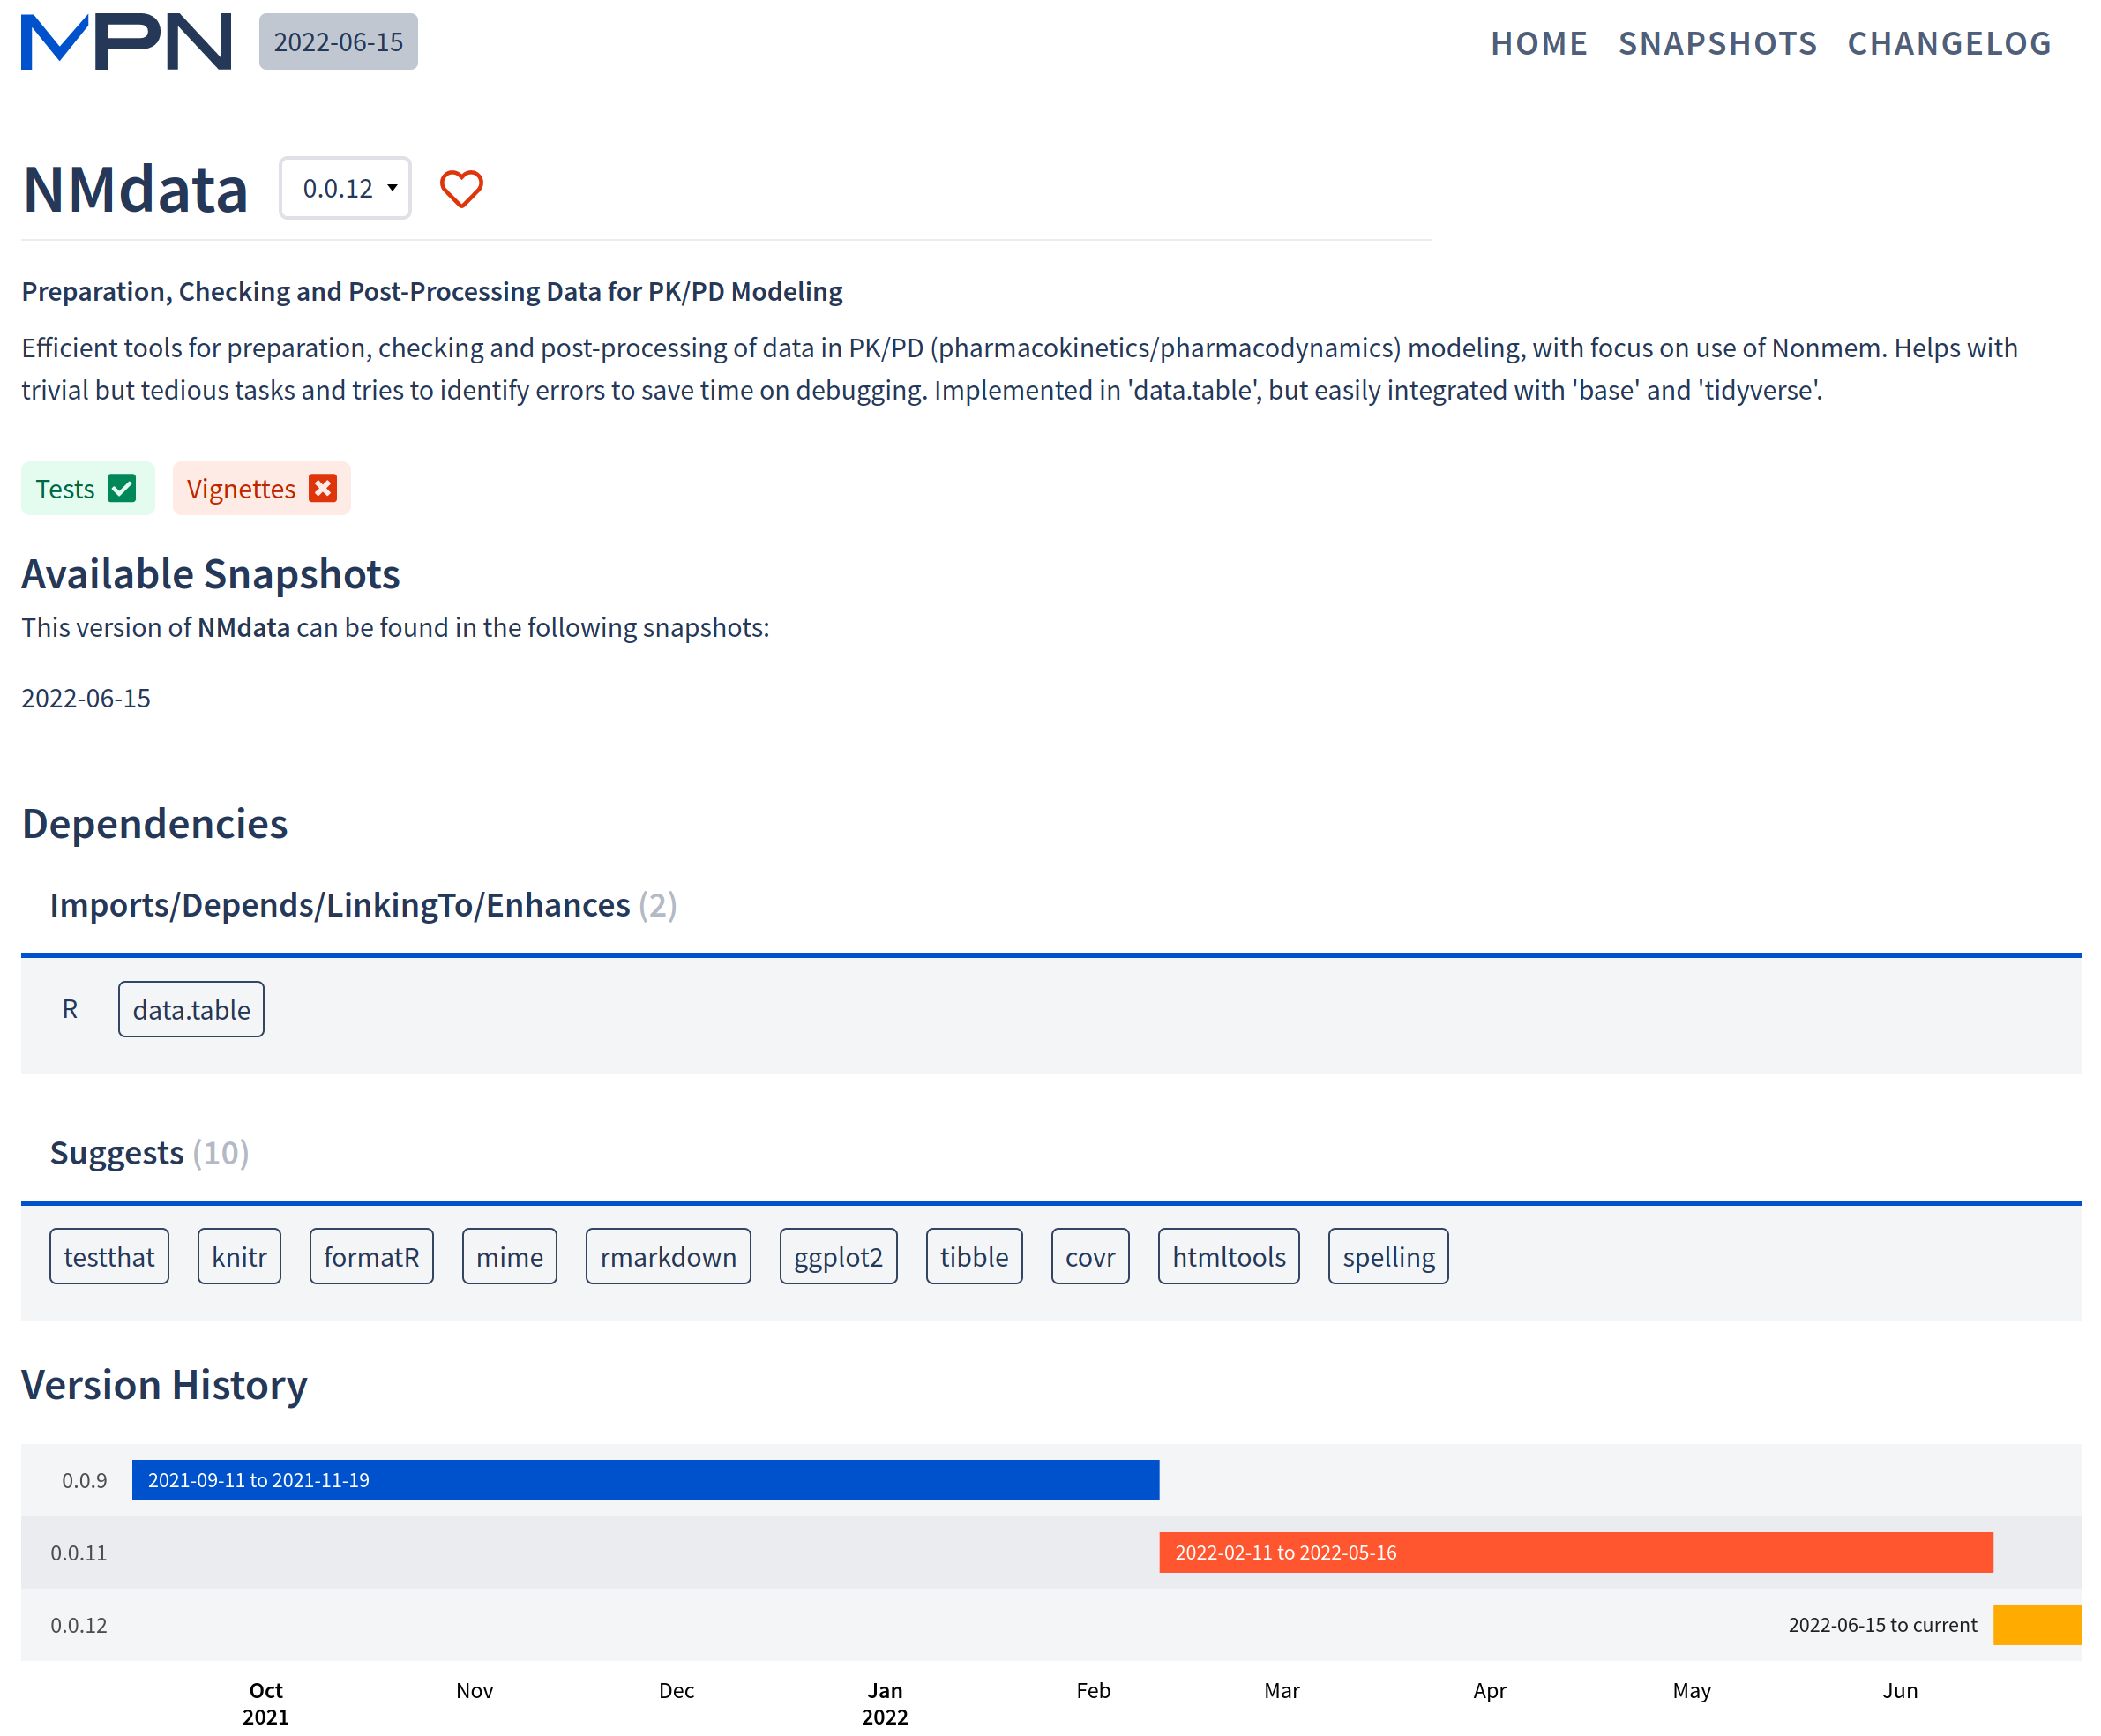
\includegraphics[width=3.5in]{figures/nmdata_mpn_2022-06-27 22-03-35.png}

\end{frame}

\begin{frame}[fragile]{How to update to recent MPN snapshot}
\protect\hypertarget{how-to-update-to-recent-mpn-snapshot}{}

Update the \texttt{pkgr.yml} file: (example:
\texttt{prod\_vx123\_001\_analysis/trunk/analysis/vx\_123\_001\_project/pkgr.yml})

\begin{verbatim}
Version: 1
Threads: 1
Packages:
  - NMdata

# this will allow packages to be cached across projects for faster installs on new projects
Cache: /data/prod_vx708_001_pkgcache-2022-06-15
Repos:
  - MPN: https://mpn.metworx.com/snapshots/stable/2022-06-15
Lockfile:
    Type: renv
\end{verbatim}

Then go to
\texttt{prod\_vx123\_001\_analysis/trunk/analysis/vx\_123\_001\_project}
and install/update packages from the linux terminal (not R):

\begin{verbatim}
$ cd /data/prod_vx123_001_analysis/trunk/analysis/vx_123_001_project
$ pkgr --update install
\end{verbatim}

\end{frame}

\begin{frame}[fragile]{Motivation}
\protect\hypertarget{motivation}{}

\begin{itemize}
\item
  The workflow of a pharmacometrician is very technical, with many risks
  of errors.
\item
  Technical workload takes time from modeling, reflection, and
  understanding key questions.
\item
  During the first 2-3 years I spent in pharmacometrics, I must have
  spent half the time coding, desparately trying to get Nonmem to
  behave, and to understand the properties of the estimates I obtained.
\item
  Most of us develop our own ways to avoid some of the many difficulties
  in this process. This takes a lot of time and is most often only
  because we don't have adequate tools at hand. Or don't know them.
\item
  I generalized some of my solutions and collected them in
  \texttt{NMdata}.
\item
  Almost every single line of code in the package is motivated by bad
  experiences. Errors, fear of errors, time wasted on debugging and
  double checking.
\item
  I have no intention of missioning these approaches to others. But if
  you find something interesting, feel free to take advantage.
\end{itemize}

\end{frame}

\begin{frame}[fragile]{Getting started}
\protect\hypertarget{getting-started}{}

Install from \texttt{CRAN} or from \texttt{MPN} using \texttt{pkgr}.

\begin{Shaded}
\begin{Highlighting}[]
\KeywordTok{library}\NormalTok{(NMdata)}
\end{Highlighting}
\end{Shaded}

\begin{verbatim}
## Welcome to NMdata. Best place to browse NMdata documentation is
## https://philipdelff.github.io/NMdata/
\end{verbatim}

Three vignettes are available so far (see ``Vignettes'' tab when
visiting URL above):

\begin{itemize}
\tightlist
\item
  \href{https://htmlpreview.github.io/?https://github.com/philipdelff/NMdata/blob/master/vignettes/NMdata-cheat.html}{Cheat
  sheet}
\item
  \href{https://philipdelff.github.io/NMdata/articles/DataCreate.html}{Data
  creation tools}
\item
  \href{https://philipdelff.github.io/NMdata/articles/NMscanData.html}{Automated
  and general reader of Nonmem data}
\item
  \href{https://philipdelff.github.io/NMdata/articles/NMdata-FAQ.html}{FAQ}
\end{itemize}

For a quick overview (after installation), do:

\begin{Shaded}
\begin{Highlighting}[]
\KeywordTok{help}\NormalTok{(}\DataTypeTok{package=}\StringTok{"NMdata"}\NormalTok{)}
\end{Highlighting}
\end{Shaded}

All functions and their arguments are documented in ?manual pages.

\end{frame}

\hypertarget{data-set-creation}{%
\section{Data set creation}\label{data-set-creation}}

\begin{frame}[fragile]{Compare compatibility of data sets for rbind and
merge: \texttt{compareCols}}
\protect\hypertarget{compare-compatibility-of-data-sets-for-rbind-and-merge-comparecols}{}

\begin{columns}[T]
\begin{column}{0.48\textwidth}
\begin{itemize}
\tightlist
\item
  In order to rbind or merge data sets, they must be compatible in
\item
  presence of columns, depending of desired outcome
\item
  equally importantly, the classes of the common columns.
\item
  \texttt{compareCols} provides an overview of these properties for any
  number of data sets.
\item
  By default, only discrepancies are returned.
\item
  Using \texttt{diff.only=FALSE} will give the complete list of columns
  in the two datasets.
\end{itemize}

A slightly modified version of the \texttt{pk} dataset has been created.

\begin{itemize}
\tightlist
\item
  Rows have been omitted
\item
  \texttt{CYCLE} has been removed, and
\item
  \texttt{AMT} has been recoded to character
\end{itemize}
\end{column}

\begin{column}{0.48\textwidth}
\begin{Shaded}
\begin{Highlighting}[]
\KeywordTok{compareCols}\NormalTok{(pk,pk.reduced)}
\end{Highlighting}
\end{Shaded}

\begin{verbatim}
## Dimensions:
\end{verbatim}

\begin{verbatim}
##          data nrows ncols
## 1:         pk  1502    22
## 2: pk.reduced   751    21
\end{verbatim}

\begin{verbatim}
## 
## Columns that differ:
\end{verbatim}

\begin{verbatim}
##    column      pk pk.reduced
## 1:  CYCLE integer       <NA>
## 2:    AMT integer  character
\end{verbatim}

\begin{verbatim}
## 
\end{verbatim}

\begin{verbatim}
## Columns where no differences were found: BLQ,
## CMT, DOSE, DV, EVENTU, EVID, FLAG, ID, NAME,
## NOMTIME, PART, PROFDAY, PROFTIME, STUDY, TIME,
## TIMEUNIT, TRTACT, WEIGHTB, eff0, flag.
\end{verbatim}

\vspace{12pt}

Before merging or stacking, we may want to

\begin{itemize}
\tightlist
\item
  recode \texttt{AMT} in one of the datasets to get the class we need
\item
  decide what to do about the missing \texttt{CYCLE} in one of the
  datasets
\end{itemize}
\end{column}
\end{columns}

\end{frame}

\begin{frame}[fragile]{Keep track of missing values}
\protect\hypertarget{keep-track-of-missing-values}{}

\begin{Shaded}
\begin{Highlighting}[]
\NormalTok{missings <-}\StringTok{ }\KeywordTok{listMissings}\NormalTok{(pk)}
\end{Highlighting}
\end{Shaded}

\begin{verbatim}
##    variable Nmissing
## 1:       DV      150
\end{verbatim}

\begin{Shaded}
\begin{Highlighting}[]
\KeywordTok{head}\NormalTok{(missings)}
\end{Highlighting}
\end{Shaded}

\begin{verbatim}
##    variable row value
## 1:       DV   1  <NA>
## 2:       DV  11  <NA>
## 3:       DV  21  <NA>
## 4:       DV  31  <NA>
## 5:       DV  41  <NA>
## 6:       DV  51  <NA>
\end{verbatim}

You can specify

\begin{itemize}
\tightlist
\item
  What columns to search
\item
  A grouping variable for findings (i.e.~study if combining datasets)
\item
  The strings that are interpreted as missing.
\end{itemize}

From \texttt{?listMissings}:

\begin{verbatim}
Usage:

     listMissings(data, cols, by, na.strings = c("", "."), quiet = FALSE, as.fun)
\end{verbatim}

\end{frame}

\begin{frame}[fragile]{Rename columns based on contents}
\protect\hypertarget{rename-columns-based-on-contents}{}

\begin{columns}[T]
\begin{column}{0.48\textwidth}
\begin{block}{renameByContents}

\begin{itemize}
\tightlist
\item
  Nonmem almost entirely relies on numeric data values.
\item
  The source data will often contain character variables, i.e.~columns
  with non-numeric data values. We want to use these and other
  non-numerics in post-processing.
\item
  If the column names reflect whether the values are numeric, mistakes
  and double-checking can be avoided.
\item
  \texttt{renameByContents} renames columns if a function of their
  contents returns \texttt{TRUE}.
\end{itemize}

\end{block}

\begin{block}{\texttt{NMisNumeric}}

\begin{itemize}
\tightlist
\item
  \texttt{NMisNumeric} is a function that tests if the contents are
  numeric to \texttt{Nonmem}.
\item
  Subject ID \texttt{"1039"} (character class) will be a numeric in
  Nonmem, \texttt{"1-039"} will not.
\item
  We invert that, and those that Nonmem cannot interpret as numeric
  become lowercase.
\end{itemize}

\end{block}
\end{column}

\begin{column}{0.48\textwidth}
All column names are capital case. We rename to lowercase those that
Nonmem will not be able to interpret as numeric. \footnotesize

\begin{Shaded}
\begin{Highlighting}[]
\NormalTok{pk <-}\StringTok{ }\KeywordTok{renameByContents}\NormalTok{(}\DataTypeTok{data=}\NormalTok{pk,}
                       \DataTypeTok{fun.test=}\NormalTok{NMisNumeric,}
                       \DataTypeTok{fun.rename =}\NormalTok{ tolower,}
                       \DataTypeTok{invert.test =} \OtherTok{TRUE}\NormalTok{)}
\end{Highlighting}
\end{Shaded}

\texttt{compareCols} shows that four columns were renamed:

\begin{Shaded}
\begin{Highlighting}[]
\KeywordTok{compareCols}\NormalTok{(pk.old,pk)}
\end{Highlighting}
\end{Shaded}

\begin{verbatim}
## Dimensions:
\end{verbatim}

\begin{verbatim}
##      data nrows ncols
## 1: pk.old  1502    22
## 2:     pk  1502    22
\end{verbatim}

\begin{verbatim}
## 
## Columns that differ:
\end{verbatim}

\begin{verbatim}
##      column    pk.old        pk
## 1:   EVENTU character      <NA>
## 2:     NAME character      <NA>
## 3: TIMEUNIT character      <NA>
## 4:   TRTACT character      <NA>
## 5:   eventu      <NA> character
## 6:     name      <NA> character
## 7: timeunit      <NA> character
## 8:   trtact      <NA> character
\end{verbatim}

\begin{verbatim}
## 
\end{verbatim}

\begin{verbatim}
## Columns where no differences were found: AMT, BLQ, CMT,
## CYCLE, DOSE, DV, EVID, FLAG, ID, NOMTIME, PART, PROFDAY,
## PROFTIME, STUDY, TIME, WEIGHTB, eff0, flag.
\end{verbatim}

\normalsize
\end{column}
\end{columns}

\end{frame}

\begin{frame}[fragile]{Automated checking of merges}
\protect\hypertarget{automated-checking-of-merges}{}

\begin{itemize}
\tightlist
\item
  Merges are a very common source of data creation bugs.
\item
  Merges likely leave you with an unexpected number of rows, some
  repeated or some omitted.
\item
  \texttt{mergeCheck} is a wrapper of \texttt{merge} which only accepts
  the results if
\end{itemize}

\textbf{The rows that come out of the merge are the exact same as in one
of the existing datasets, only columns added from the second dataset}

\begin{itemize}
\item
  This limitation of the scope of the merge allows for a high degree of
  automated checks of consistency of the results.
\item
  This is not to say that merges beyond the scope of \texttt{mergeCheck}
  are relevant or necessary. But if \texttt{mergeCheck} covers your
  needs, it's a real time saver in terms of automated checks.
\end{itemize}

\textbf{mergeCheck is not a new implementation of merge. It's an
implementation of checks.}

\begin{itemize}
\item
  \texttt{mergeCheck} uses \texttt{merge.data.table}. The contribution
  is the checks that no rows are lost, duplicated or added.
\item
  The order of rows in the resulting data is always the same as the
  first dataset supplied.
\end{itemize}

Is \texttt{mergeCheck} slower?

\begin{itemize}
\tightlist
\item
  If you don't use data.table already, \texttt{mergeCheck} is likely to
  be way faster than what you use already.
\item
  The checking overlay should be neglegible.
\item
  If checks fail, an additional merge is done to help user identify
  problems. This may cost significant additional time but is likely to
  save you coding and (at least) the same calculation time anyway.
\end{itemize}

\end{frame}

\begin{frame}[fragile]{mergeCheck}
\protect\hypertarget{mergecheck}{}

\framesubtitle{Example: Would your standard checks of merges capture this?}

Say we want to add a covariate from a \texttt{dt.cov}. We expect the
number of rows to be unchanged from \texttt{pk}. \texttt{mergeCheck}
more strictly requires that we get all and only the \emph{same} rows:

\begin{columns}[T]
\begin{column}{0.48\textwidth}
\begin{block}{Without \texttt{mergeCheck}}

\footnotesize

\begin{Shaded}
\begin{Highlighting}[]
\CommentTok{## The resulting dimensions are correct}
\NormalTok{pkmerge <-}\StringTok{ }\KeywordTok{merge}\NormalTok{(pk,dt.cov,}\DataTypeTok{by=}\StringTok{"ID"}\NormalTok{)}
\KeywordTok{dims}\NormalTok{(pk,dt.cov,pkmerge)}
\end{Highlighting}
\end{Shaded}

\begin{verbatim}
##       data nrows ncols
## 1:      pk  1502    22
## 2:  dt.cov   150     2
## 3: pkmerge  1502    23
\end{verbatim}

\begin{Shaded}
\begin{Highlighting}[]
\CommentTok{## But we now have twice as many rows for this subject}
\KeywordTok{dims}\NormalTok{(pk[ID}\OperatorTok{==}\DecValTok{31}\NormalTok{],pkmerge[ID}\OperatorTok{==}\DecValTok{31}\NormalTok{])}
\end{Highlighting}
\end{Shaded}

\begin{verbatim}
##                 data nrows ncols
## 1:      pk[ID == 31]    10    22
## 2: pkmerge[ID == 31]    20    23
\end{verbatim}

\end{block}
\end{column}

\begin{column}{0.48\textwidth}
\begin{block}{\texttt{mergeCheck} throws an error}

\ldots{}and suggests what is wrong \footnotesize

\begin{Shaded}
\begin{Highlighting}[]
\KeywordTok{try}\NormalTok{(}\KeywordTok{mergeCheck}\NormalTok{(pk,dt.cov,}\DataTypeTok{by=}\StringTok{"ID"}\NormalTok{)) }
\end{Highlighting}
\end{Shaded}

\begin{verbatim}
## Rows disappeared during merge.
\end{verbatim}

\begin{verbatim}
## Rows duplicated during merge.
\end{verbatim}

\begin{verbatim}
## Overview of dimensions of input and output data:
##    nrows ncols
## 1:  1502    22
## 2:   150     2
## 3:  1502    23
\end{verbatim}

\begin{verbatim}
## Overview of values of by where number of rows in x changes:
##     ID N.x N.result
## 1:  31  10       20
## 2: 180  10        0
\end{verbatim}

\begin{verbatim}
## Error in mergeCheck(pk, dt.cov, by = "ID") : 
##   Merge added and/or removed rows.
\end{verbatim}

\end{block}
\end{column}

\normalsize
\end{columns}

\begin{block}{Conclusion}

If you only want to add columns by a merge, \texttt{mergeCheck} does all
the necessary checks for you.

\end{block}

\end{frame}

\begin{frame}[fragile]{Exclusion flags}
\protect\hypertarget{exclusion-flags}{}

\framesubtitle{Keep track of data exclusions - don't discard!}

\begin{itemize}
\item
  It is good practice not to discard unwanted records from a dataset but
  to flag them and omit them in model estimation.
\item
  When reporting the analysis, we need to account for how many data
  records were discarded due to which criteria.
\item
  The implementation in \texttt{NMdata} is based on sequentially
  checking exclusion conditions.
\item
  The information is represented in one numerical column for Nonmem, and
  one (value-to-value corresponding) character column for the rest of
  us.
\end{itemize}

\end{frame}

\begin{frame}[fragile]{FlagsAssign}
\protect\hypertarget{flagsassign}{}

\begin{columns}[T]
\begin{column}{0.48\textwidth}
\begin{itemize}
\tightlist
\item
  \texttt{flagsAssign} applies the conditions sequentially, by
  increasing or decreasing value of \texttt{FLAG}.
\item
  You can use any expression that can be evaluated \emph{row-wise}
  within the data.frame. In this case, \texttt{BLQ} has to exist in
  \texttt{pk}.
\item
  If you need to evaluate a condition based on multiple rows (say
  inadequate dosing history for a subject), do that first, and include a
  column representing this condition.
\item
  \texttt{FLAG=0} means that none of the conditions were met and row is
  kept in analysis. This cannot be customized.
\item
  In \texttt{Nonmem}, you can include \texttt{IGNORE=(FLAG.NE.0)} in
  \texttt{\$DATA} or \texttt{\$INFILE}.
\end{itemize}
\end{column}

\begin{column}{0.48\textwidth}
\footnotesize

\begin{Shaded}
\begin{Highlighting}[]
\NormalTok{dt.flags <-}\StringTok{ }\KeywordTok{fread}\NormalTok{(}\DataTypeTok{text=}\StringTok{"FLAG,flag,condition}
\StringTok{10,Below LLOQ,BLQ==1}
\StringTok{100,Negative time,TIME<0"}\NormalTok{)}

\NormalTok{pk <-}\StringTok{ }\KeywordTok{flagsAssign}\NormalTok{(pk,}\DataTypeTok{tab.flags=}\NormalTok{dt.flags,}\DataTypeTok{subset.data=}\StringTok{"EVID==0"}\NormalTok{)}
\end{Highlighting}
\end{Shaded}

\begin{verbatim}
## Coding FLAG = 100, flag = Negative time
\end{verbatim}

\begin{verbatim}
## Coding FLAG = 10, flag = Below LLOQ
\end{verbatim}

\begin{Shaded}
\begin{Highlighting}[]
\NormalTok{pk <-}\StringTok{ }\KeywordTok{flagsAssign}\NormalTok{(pk,}\DataTypeTok{subset.data=}\StringTok{"EVID==1"}\NormalTok{,}\DataTypeTok{flagc.0=}\StringTok{"Dosing"}\NormalTok{)}
\end{Highlighting}
\end{Shaded}
\end{column}
\end{columns}

\end{frame}

\begin{frame}[fragile]{\texttt{flagsCount}}
\protect\hypertarget{flagscount}{}

\begin{itemize}
\item
  An overview of the number of observations disregarded due to the
  different conditions is then obtained using \texttt{flagsCount}:
\item
  \texttt{flagsCount} includes a \texttt{file} argument to save the the
  table right away.
\end{itemize}

\footnotesize

\begin{Shaded}
\begin{Highlighting}[]
\KeywordTok{flagsCount}\NormalTok{(}\DataTypeTok{data=}\NormalTok{pk[EVID}\OperatorTok{==}\DecValTok{0}\NormalTok{],}\DataTypeTok{tab.flags=}\NormalTok{dt.flags)}
\end{Highlighting}
\end{Shaded}

\begin{verbatim}
##                  flag N.left Nobs.left N.discard N.disc.cum Nobs.discard Nobs.disc.cum
## 1: All available data    150      1352        NA          0           NA             0
## 2:      Negative time    150      1350         0          0            2             2
## 3:         Below LLOQ    131       755        19         19          595           597
## 4:       Analysis set    131       755        NA         19           NA           597
\end{verbatim}

\begin{itemize}
\tightlist
\item
  Now pick the columns you want and format your table for the report.
\end{itemize}

\end{frame}

\hypertarget{finalize-data-for-nonmem}{%
\section{Finalize data for Nonmem}\label{finalize-data-for-nonmem}}

\begin{frame}[fragile]{Advice: always include a unique row identifier}
\protect\hypertarget{advice-always-include-a-unique-row-identifier}{}

\begin{columns}[T]
\begin{column}{0.48\textwidth}
\begin{block}{Why}

A unique identifier is needed in order to

\begin{itemize}
\item
  Track rows in analysis data back to source data
\item
  Reliably combine (by merge) output with input data
\end{itemize}

\end{block}

\begin{block}{The identifier should be}

\begin{itemize}
\item
  Numeric
\item
  For Nonmem to be able to read it
\item
  Integer
\item
  To avoid risk of rounding
\item
  It is \emph{not} a problem if represented as a \texttt{double} in
  \texttt{R}
\item
  Increasing
\item
  Not strictly necessary
\item
  Avoid confusion
\item
  May be useful for post-processing to have a single column to order by
\end{itemize}

\end{block}
\end{column}

\begin{column}{0.48\textwidth}
\begin{block}{Sort rows and add a row counter}

\begin{itemize}
\tightlist
\item
  with \texttt{data.table}
\end{itemize}

\begin{Shaded}
\begin{Highlighting}[]
\CommentTok{## order}
\KeywordTok{setorder}\NormalTok{(pk,ID,TIME,EVID)}
\CommentTok{## add counter}
\NormalTok{pk[,ROW}\OperatorTok{:}\ErrorTok{=}\NormalTok{.I]}
\end{Highlighting}
\end{Shaded}

\begin{itemize}
\tightlist
\item
  Or, with \texttt{dplyr} (I'm not very familiar with \texttt{dplyr})
\end{itemize}

\begin{Shaded}
\begin{Highlighting}[]
\NormalTok{pk <-}\StringTok{ }\NormalTok{pk }\OperatorTok
\StringTok{    }\KeywordTok{arrange}\NormalTok{(ID,TIME,EVID) }\OperatorTok
\StringTok{    }\KeywordTok{mutate}\NormalTok{(}\DataTypeTok{ROW=}\DecValTok{1}\OperatorTok{:}\KeywordTok{n}\NormalTok{())}
\end{Highlighting}
\end{Shaded}

\end{block}
\end{column}
\end{columns}

\end{frame}

\begin{frame}[fragile]{NMorderColumns}
\protect\hypertarget{nmordercolumns}{}

\begin{columns}[T]
\begin{column}{0.48\textwidth}
\vspace{12pt}

\begin{itemize}
\item
  The order of columns in Nonmem is important for two reasons.
\item
  Non-numeric Characters in a variable read into Nonmem will make the
  run fail
\item
  The number of variables you can read into Nonmem is restricted (may
  not apply to recent Nonmem versions)
\item
  \texttt{NMorderColumns} uses a mix of recognition of column names and
  analysis of the column contents to sort the columns.
\item
  First: Standard columns (\texttt{ID}, \texttt{TIME}, \texttt{EVID}
  etc.) and usable columns first
\item
  Columns that cannot be converted to numeric are put in the back
\item
  Additional columns to place earlier (argument \texttt{first}) or late
  (\texttt{last}) can be specified.
\item
  See \texttt{?NMorderColumns} for more options.
\item
  \texttt{NMorderColumns} does not sort rows, nor does it modify any
  contents of columns.
\end{itemize}
\end{column}

\begin{column}{0.48\textwidth}
\footnotesize

\begin{Shaded}
\begin{Highlighting}[]
\NormalTok{pk.old <-}\StringTok{ }\KeywordTok{copy}\NormalTok{(pk)}
\NormalTok{pk <-}\StringTok{ }\KeywordTok{NMorderColumns}\NormalTok{(pk,}\DataTypeTok{first=}\StringTok{"WEIGHTB"}\NormalTok{)}
\end{Highlighting}
\end{Shaded}

\normalsize

We may want to add \texttt{MDV} and rerun \texttt{NMorderColumns}.
\footnotesize

\begin{Shaded}
\begin{Highlighting}[]
\KeywordTok{data.table}\NormalTok{(}\DataTypeTok{old=}\KeywordTok{colnames}\NormalTok{(pk.old),}\DataTypeTok{new=}\KeywordTok{colnames}\NormalTok{(pk))}
\end{Highlighting}
\end{Shaded}

\begin{verbatim}
##          old      new
##  1:       ID      ROW
##  2:  NOMTIME       ID
##  3:     TIME  NOMTIME
##  4:     EVID     TIME
##  5:      CMT     EVID
##  6:      AMT      CMT
##  7:       DV      AMT
##  8:    STUDY       DV
##  9:      BLQ  WEIGHTB
## 10:    CYCLE     FLAG
## 11:     DOSE    STUDY
## 12:     PART      BLQ
## 13:  PROFDAY    CYCLE
## 14: PROFTIME     DOSE
## 15:  WEIGHTB     PART
## 16:     eff0  PROFDAY
## 17:   eventu PROFTIME
## 18:     name     eff0
## 19: timeunit   eventu
## 20:   trtact     flag
## 21:     FLAG     name
## 22:     flag timeunit
## 23:      ROW   trtact
##          old      new
\end{verbatim}
\end{column}

\normalsize
\end{columns}

\end{frame}

\begin{frame}[fragile]{\texttt{NMcheckData}: Check data syntax for
Nonmem compatibility}
\protect\hypertarget{nmcheckdata-check-data-syntax-for-nonmem-compatibility}{}

\begin{itemize}
\item
  Aim: check data for all potential Nonmem compatibility issues and
  other obvious errors.
\item
  Findings must be returned in a structure so related subsets of the
  data can easily be identified for further inspection.
\end{itemize}

\begin{columns}[T]
\begin{column}{0.48\textwidth}
\begin{itemize}
\item
  \texttt{NMcheckData} contains a very long list of checks of especially
  the standard Nonmem columns (\texttt{ID}, \texttt{TIME},
  \texttt{EVID}, \texttt{AMT}, \texttt{DV}, \texttt{MDV}, \texttt{RATE},
  \texttt{SS}, etc.). They are all checked for allowed values (e.g.
  \texttt{TIME} must be non-negative, \texttt{EVID} must be one of
  \texttt{0:4}, etc).
\item
  ID-level checks (e.g.~did all ID's receive doses, is time increasing,
  are rows disjoint?)
\item
  All used columns are checked for Nonmem compatibility in terms of how
  Nonmem translates to numeric values.
\item
  Column names are checked for uniqueness and for non-allowed
  characters.
\item
  If you supply the col.usubjid column, the ID column is checked to
  align with col.usubjid.
\item
  \texttt{NMcheckData} is based on simple framework making it simple to
  define new checks.
\end{itemize}
\end{column}

\begin{column}{0.48\textwidth}
\scriptsize

\begin{Shaded}
\begin{Highlighting}[]
\NormalTok{pk <-}\StringTok{ }\NormalTok{pk[ID}\OperatorTok{>}\DecValTok{59}\NormalTok{]}
\NormalTok{res.check <-}\StringTok{ }\KeywordTok{NMcheckData}\NormalTok{(pk)}
\end{Highlighting}
\end{Shaded}

\begin{verbatim}
##  column              check N Nid
##    EVID Subject has no obs 1   1
##     MDV   Column not found 1   0
\end{verbatim}

\begin{Shaded}
\begin{Highlighting}[]
\NormalTok{res.check}
\end{Highlighting}
\end{Shaded}

\begin{verbatim}
##    row ID column              check  level ROW
## 1:  NA 60   EVID Subject has no obs     ID  NA
## 2:  NA NA    MDV   Column not found column  NA
\end{verbatim}

\begin{Shaded}
\begin{Highlighting}[]
\NormalTok{pkmod <-}\StringTok{ }\KeywordTok{copy}\NormalTok{(pk)}
\NormalTok{pkmod[,MDV}\OperatorTok{:}\ErrorTok{=}\KeywordTok{as.numeric}\NormalTok{(}\KeywordTok{is.na}\NormalTok{(DV))]}
\NormalTok{pkmod[ID}\OperatorTok{==}\DecValTok{60}\OperatorTok{&}\NormalTok{EVID}\OperatorTok{==}\DecValTok{1}\NormalTok{,CMT}\OperatorTok{:}\ErrorTok{=}\OtherTok{NA}\NormalTok{]}
\NormalTok{res.check <-}\StringTok{ }\KeywordTok{NMcheckData}\NormalTok{(pkmod)}
\end{Highlighting}
\end{Shaded}

\begin{verbatim}
##  column               check N Nid
##    EVID  Subject has no obs 1   1
##     CMT Missing for EVID!=3 1   1
\end{verbatim}

\begin{Shaded}
\begin{Highlighting}[]
\NormalTok{res.check}
\end{Highlighting}
\end{Shaded}

\begin{verbatim}
##    row ID column               check level ROW
## 1:  NA 60   EVID  Subject has no obs    ID  NA
## 2:   1 60    CMT Missing for EVID!=3   row 291
\end{verbatim}
\end{column}
\end{columns}

\end{frame}

\begin{frame}[fragile]{NMwriteData}
\protect\hypertarget{nmwritedata}{}

\begin{columns}[T]
\begin{column}{0.48\textwidth}
For the final step of writing the dataset, \texttt{NMwriteData} is
provided.

\begin{itemize}
\item
  \texttt{NMwriteData} \emph{never} modifies the data.
\item
  Checks character variables for Nonmem compatibility (commas not
  allowed)
\item
  writes a \texttt{csv} file with appropriate options for Nonmem
  compatibility
\item
  Default is to also write an \texttt{rds} file for R
\item
  Contents identical to R object including all information (such as
  factor levels) which cannot be saved in csv.
\item
  If you use \texttt{NMscanData} to read Nonmem results, this
  information can be used automatically.
\item
  Provides a proposal for text to include in the \texttt{\$INPUT} and
  \texttt{\$DATA} sections of the Nonmem control streams.
\end{itemize}

\begin{block}{The csv writer is very simple}

These are the only steps involved between the supplied data set and the
written csv.

\begin{itemize}
\tightlist
\item
  \texttt{scipen} is small to maximize precision.
\end{itemize}

\footnotesize

\begin{Shaded}
\begin{Highlighting}[]
\NormalTok{file.csv <-}\StringTok{ }\KeywordTok{fnExtension}\NormalTok{(file,}\StringTok{".csv"}\NormalTok{)}
\KeywordTok{fwrite}\NormalTok{(data,}\DataTypeTok{na=}\StringTok{"."}\NormalTok{,}\DataTypeTok{quote=}\OtherTok{FALSE}\NormalTok{,}\DataTypeTok{row.names=}\OtherTok{FALSE}\NormalTok{,}\DataTypeTok{scipen=}\DecValTok{0}\NormalTok{,}\DataTypeTok{file=}\NormalTok{file.csv)}
\end{Highlighting}
\end{Shaded}

\normalsize

All arguments to \texttt{fwrite} can be modified using the
\texttt{args.fwrite} argument.

\end{block}
\end{column}

\begin{column}{0.48\textwidth}
\footnotesize

\begin{Shaded}
\begin{Highlighting}[]
\KeywordTok{NMwriteData}\NormalTok{(pk,}\DataTypeTok{file=}\StringTok{"derived/pk.csv"}\NormalTok{)}
\end{Highlighting}
\end{Shaded}

\begin{verbatim}
## Data written to file(s):
## derived/pk.csv
## derived/pk.rds
\end{verbatim}

\begin{verbatim}
## For NONMEM:
## $INPUT ROW ID NOMTIME TIME EVID CMT AMT DV WEIGHTB
## FLAG STUDY BLQ CYCLE DOSE PART PROFDAY PROFTIME eff0
## $DATA derived/pk.csv
## IGN=@
## IGNORE=(FLAG.NE.0)
\end{verbatim}

\normalsize

\vspace{12pt}

\begin{itemize}
\item
  \texttt{eff0} is the last column in \texttt{pk} that \texttt{Nonmem}
  can make use of (remember \texttt{NMisNumeric} from earlier?)
\item
  \texttt{NMwriteData} detected the exclusion flag and suggests to
  include it in \texttt{\$DATA}.
\end{itemize}
\end{column}
\end{columns}

\end{frame}

\begin{frame}[fragile]{Update Nonmem control streams}
\protect\hypertarget{update-nonmem-control-streams}{}

\begin{columns}[T]
\begin{column}{0.48\textwidth}
\begin{itemize}
\item
  \texttt{NMwriteSection} is a function that replaces sections (like
  \$DATA or \$TABLE) of nonmem control streams.
\item
  \texttt{NMwriteData} returns a list that can be directly processed by
  \texttt{NMwriteSection}
\item
  In \texttt{NMwriteData}, several arguments modify the proposed text
  the proposed text for the Nonmem run, see \texttt{?NMwriteData}.
\end{itemize}

\begin{block}{Tips}

\begin{itemize}
\item
  \texttt{NMwriteData} is very useful for many other sections, like
  \texttt{\$TABLE}, or even \texttt{\$PK}. But not \texttt{\$THETA} and
  \texttt{\$OMEAGE} (because they are specific to each model).
\item
  \texttt{NMwriteData} by defaults saves a backup of the overwritten
  control streams.
\item
  \texttt{NMwriteData} has a section \emph{reader} counterpart in
  \texttt{NMreadSection}
\item
  \texttt{NMextractDataFile} takes a control stream/list file and
  extracts the input data file name/path. You can use this to identify
  the model runs in which to update \texttt{\$DATA}.
\end{itemize}

\end{block}
\end{column}

\begin{column}{0.48\textwidth}
\footnotesize

\begin{Shaded}
\begin{Highlighting}[]
\NormalTok{nmCode <-}\StringTok{ }\KeywordTok{NMwriteData}\NormalTok{(pk,}\DataTypeTok{file=}\StringTok{"derived/pk.csv"}\NormalTok{,}
                      \DataTypeTok{write.csv=}\OtherTok{FALSE}\NormalTok{,}
\CommentTok{### arguments that tailors text for Nonmem}
                      \DataTypeTok{nmdir.data=}\StringTok{"../derived"}\NormalTok{,}
                      \DataTypeTok{nm.drop=}\StringTok{"PROFDAY"}\NormalTok{,}
                      \DataTypeTok{nm.copy=}\KeywordTok{c}\NormalTok{(}\DataTypeTok{CONC=}\StringTok{"DV"}\NormalTok{),}
                      \DataTypeTok{nm.rename=}\KeywordTok{c}\NormalTok{(}\DataTypeTok{BBW=}\StringTok{"WEIGHTB"}\NormalTok{),}
                      \CommentTok{## PSN compatibility}
                      \DataTypeTok{nm.capitalize=}\OtherTok{TRUE}\NormalTok{)}
\end{Highlighting}
\end{Shaded}

\begin{verbatim}
## Data _not_ witten to any files.
\end{verbatim}

\begin{verbatim}
## For NONMEM:
## $INPUT ROW ID NOMTIME TIME EVID CMT AMT CONC=DV BBW
## FLAG STUDY BLQ CYCLE DOSE PART PROFDAY=DROP PROFTIME
## EFF0
## $DATA ../derived/pk.csv
## IGN=@
## IGNORE=(FLAG.NE.0)
\end{verbatim}

\begin{Shaded}
\begin{Highlighting}[]
\CommentTok{## example: pick run1*.mod}
\KeywordTok{NMwriteSection}\NormalTok{(}\DataTypeTok{dir=}\StringTok{"../models"}\NormalTok{,}
               \DataTypeTok{file.pattern=}\StringTok{"run1.+}\CharTok{\textbackslash{}\textbackslash{}}\StringTok{.mod$"}\NormalTok{,}
               \DataTypeTok{section=}\StringTok{"INPUT"}\NormalTok{,}
               \DataTypeTok{newlines=}\NormalTok{nmCode}\OperatorTok{$}\NormalTok{INPUT)}
\end{Highlighting}
\end{Shaded}

\normalsize
\end{column}
\end{columns}

\end{frame}

\begin{frame}[fragile]{Automated documentation of data}
\protect\hypertarget{automated-documentation-of-data}{}

\framesubtitle{Ensure that the data can be traced back to the data generation script}

\begin{columns}[T]
\begin{column}{0.48\textwidth}
\begin{itemize}
\item
  If the argument \texttt{script} is supplied to \texttt{NMwriteData}, a
  little meta information is saved together with the output file(s).
\item
  For csv files, the meta data is written to a txt file next to the csv
  file.
\item
  For rds files, the meta data is attached to the object saved in the
  \texttt{rds} file.
\item
  \texttt{NMstamp} is used under the hood. You can use \texttt{NMstamp}
  on any R object to attach similar meta information.
\item
  Additional arguments (essentially anything) can be passed from
  \texttt{NMwriteData} to \texttt{NMstamp} using the argument
  \texttt{args.stamp}.
\item
  \texttt{NMstamp} and \texttt{NMinfo} write and read an ``attribute''
  called \texttt{NMdata}.
\end{itemize}
\end{column}

\begin{column}{0.48\textwidth}
\footnotesize

\begin{Shaded}
\begin{Highlighting}[]
\KeywordTok{NMwriteData}\NormalTok{(pk,}\DataTypeTok{file=}\StringTok{"derived/pk.csv"}\NormalTok{,}
            \DataTypeTok{script =} \StringTok{"NMdata_Rpackage.Rmd"}\NormalTok{,}\DataTypeTok{quiet=}\NormalTok{T)}
\KeywordTok{list.files}\NormalTok{(}\StringTok{"derived"}\NormalTok{)}
\end{Highlighting}
\end{Shaded}

\begin{verbatim}
## [1] "pk_meta.txt" "pk.csv"      "pk.rds"
\end{verbatim}

\begin{Shaded}
\begin{Highlighting}[]
\CommentTok{## NMreadCsv reads the metadata .txt file if found}
\NormalTok{pknm <-}\StringTok{ }\KeywordTok{NMreadCsv}\NormalTok{(}\StringTok{"derived/pk.csv"}\NormalTok{)}
\KeywordTok{NMinfo}\NormalTok{(pknm)}
\end{Highlighting}
\end{Shaded}

\begin{verbatim}
## $dataCreate
## $dataCreate$DataCreateScript
## [1] "NMdata_Rpackage.Rmd"
## 
## $dataCreate$CreationTime
## [1] "2022-06-30 13:44:28 EDT"
## 
## $dataCreate$writtenTo
## [1] "derived/pk.csv"
\end{verbatim}

\begin{Shaded}
\begin{Highlighting}[]
\CommentTok{## The .rds file contains the metadata already}
\NormalTok{pknm2 <-}\StringTok{ }\KeywordTok{readRDS}\NormalTok{(}\StringTok{"derived/pk.rds"}\NormalTok{)}
\KeywordTok{NMinfo}\NormalTok{(pknm2)}
\end{Highlighting}
\end{Shaded}

\begin{verbatim}
## $dataCreate
## $dataCreate$DataCreateScript
## [1] "NMdata_Rpackage.Rmd"
## 
## $dataCreate$CreationTime
## [1] "2022-06-30 13:44:28 EDT"
## 
## $dataCreate$writtenTo
## [1] "derived/pk.rds"
\end{verbatim}
\end{column}
\end{columns}

\normalsize

\end{frame}

\hypertarget{retrieving-data-from-nonmem-runs}{%
\section{Retrieving data from Nonmem
runs}\label{retrieving-data-from-nonmem-runs}}

\begin{frame}[fragile]{NMscanData}
\protect\hypertarget{nmscandata}{}

\texttt{NMscanData} is an automated and general reader of Nonmem.

\begin{itemize}
\tightlist
\item
  Returns one data set combining all information from input data and all
  output tables. Performs multiple consistency checks.
\end{itemize}

Based on the list file (\texttt{.lst}) it will:

\begin{itemize}
\tightlist
\item
  Read and combine output tables
\item
  If wanted, read input data and restore variables that were not output
  from the \texttt{Nonmem} model
\item
  If wanted, also restore rows from input data that were disregarded in
  \texttt{Nonmem} (e.g.~observations or subjects that are not part of
  the analysis)
\end{itemize}

\pause
\footnotesize

\begin{columns}[T]
\begin{column}{0.48\textwidth}
\begin{Shaded}
\begin{Highlighting}[]
\NormalTok{file1.lst <-}\StringTok{ }\KeywordTok{system.file}\NormalTok{(}\StringTok{"examples/nonmem/xgxr003.lst"}\NormalTok{,}
                         \DataTypeTok{package=}\StringTok{"NMdata"}\NormalTok{)}
\NormalTok{res0 <-}\StringTok{ }\KeywordTok{NMscanData}\NormalTok{(file1.lst,}\DataTypeTok{merge.by.row=}\OtherTok{FALSE}\NormalTok{)}
\end{Highlighting}
\end{Shaded}

\begin{verbatim}
## No missing values identified
\end{verbatim}

\begin{verbatim}
## Model:  xgxr003 
## 
## Used tables, contents shown as used/total:
##                  file     rows columns     IDs
##       xgxr003_res.txt  905/905     7/7 150/150
##  xgxr003_res_vols.txt  905/905     3/7 150/150
##    xgxr003_res_fo.txt  150/150     1/2 150/150
##     xgxr1.csv (input) 905/1502   21/24 150/150
##              (result)      905    32+2     150
\end{verbatim}

\begin{verbatim}
## Input and output data combined by translation of
## Nonmem data filters (not recommended).
\end{verbatim}

\begin{verbatim}
## 
## Distribution of rows on event types in returned data:
##  EVID CMT output result
##     0   2    755    755
##     1   1    150    150
##   All All    905    905
\end{verbatim}
\end{column}

\pause

\begin{column}{0.48\textwidth}
\begin{Shaded}
\begin{Highlighting}[]
\KeywordTok{class}\NormalTok{(res0)}
\end{Highlighting}
\end{Shaded}

\begin{verbatim}
## [1] "NMdata"     "data.table" "data.frame"
\end{verbatim}

\begin{Shaded}
\begin{Highlighting}[]
\KeywordTok{dims}\NormalTok{(res0)}
\end{Highlighting}
\end{Shaded}

\begin{verbatim}
##    data nrows ncols
## 1: res0   905    34
\end{verbatim}

\begin{Shaded}
\begin{Highlighting}[]
\KeywordTok{head}\NormalTok{(res0,}\DataTypeTok{n=}\DecValTok{2}\NormalTok{)}
\end{Highlighting}
\end{Shaded}

\begin{verbatim}
##    ROW ID NOMTIME TIME EVID CMT AMT DV FLAG STUDY     KA
## 1:   1 31       0    0    1   1   3  0    0     1 0.1812
## 2:  11 32       0    0    1   1   3  0    0     1 0.1812
##          Q PRED RES WRES    V2     V3 BLQ CYCLE DOSE PART
## 1: 2307400    0   0    0 0.042 0.1785   0     1    3    1
## 2: 2307400    0   0    0 0.042 0.1785   0     1    3    1
##    PROFDAY PROFTIME WEIGHTB   eff0        CL EVENTU   NAME
## 1:       1        0  87.031 56.461 0.7245691     mg Dosing
## 2:       1        0 100.620 45.096 0.7245691     mg Dosing
##    TIMEUNIT TRTACT   flag trtact   model nmout
## 1:    Hours   3 mg Dosing   3 mg xgxr003  TRUE
## 2:    Hours   3 mg Dosing   3 mg xgxr003  TRUE
\end{verbatim}

\normalsize
\end{column}
\end{columns}

\end{frame}

\begin{frame}[fragile]{Remember the unique row identifier}
\protect\hypertarget{remember-the-unique-row-identifier}{}

Using a unique row identifier for merging data is highly recommended:

\footnotesize

\begin{Shaded}
\begin{Highlighting}[]
\NormalTok{res1 <-}\StringTok{ }\KeywordTok{NMscanData}\NormalTok{(}\KeywordTok{file.nm}\NormalTok{(}\StringTok{"xgxr001.lst"}\NormalTok{),}\DataTypeTok{merge.by.row=}\OtherTok{TRUE}\NormalTok{)}
\end{Highlighting}
\end{Shaded}

\begin{verbatim}
## Model:  xgxr001 
## 
## Used tables, contents shown as used/total:
##               file     rows columns     IDs
##    xgxr001_res.txt  905/905   16/16 150/150
##  xgxr1.csv (input) 905/1502   22/24 150/150
##           (result)      905    38+2     150
## 
## Input and output data merged by: ROW 
## 
## Distribution of rows on event types in returned data:
##  EVID CMT output result
##     0   2    755    755
##     1   1    150    150
##   All All    905    905
\end{verbatim}

\begin{Shaded}
\begin{Highlighting}[]
\KeywordTok{class}\NormalTok{(res0)}
\end{Highlighting}
\end{Shaded}

\begin{verbatim}
## [1] "NMdata"     "data.table" "data.frame"
\end{verbatim}

\normalsize

\begin{itemize}
\tightlist
\item
  The default behavior will be to merge by \texttt{col.row} if found.
\item
  Default value of \texttt{col.row} is \texttt{ROW}. We shall see later
  how to modify this.
\end{itemize}

\end{frame}

\begin{frame}[fragile]{NMscanData}
\protect\hypertarget{nmscandata-1}{}

\framesubtitle{Example: quickly get from a list file to looking at the model}

\footnotesize

\begin{columns}[T]
\begin{column}{0.45\textwidth}
\begin{Shaded}
\begin{Highlighting}[]
\CommentTok{## Using data.table for easy summarize}
\NormalTok{res1 <-}\StringTok{ }\KeywordTok{NMscanData}\NormalTok{(file1.lst,}\DataTypeTok{merge.by.row=}\OtherTok{TRUE}\NormalTok{,}
                   \DataTypeTok{as.fun=}\StringTok{"data.table"}\NormalTok{,}\DataTypeTok{quiet=}\OtherTok{TRUE}\NormalTok{)}
\CommentTok{## Derive geometric mean pop predictions by}
\CommentTok{## treatment and nominal sample time. Only}
\CommentTok{## use sample records.}
\NormalTok{res1[EVID}\OperatorTok{==}\DecValTok{0}\NormalTok{,}
\NormalTok{     gmPRED}\OperatorTok{:}\ErrorTok{=}\KeywordTok{exp}\NormalTok{(}\KeywordTok{mean}\NormalTok{(}\KeywordTok{log}\NormalTok{(PRED))),}
\NormalTok{     by=.(trtact,NOMTIME)]}
\end{Highlighting}
\end{Shaded}
\end{column}

\begin{column}{0.55\textwidth}
\normalsize

\begin{center}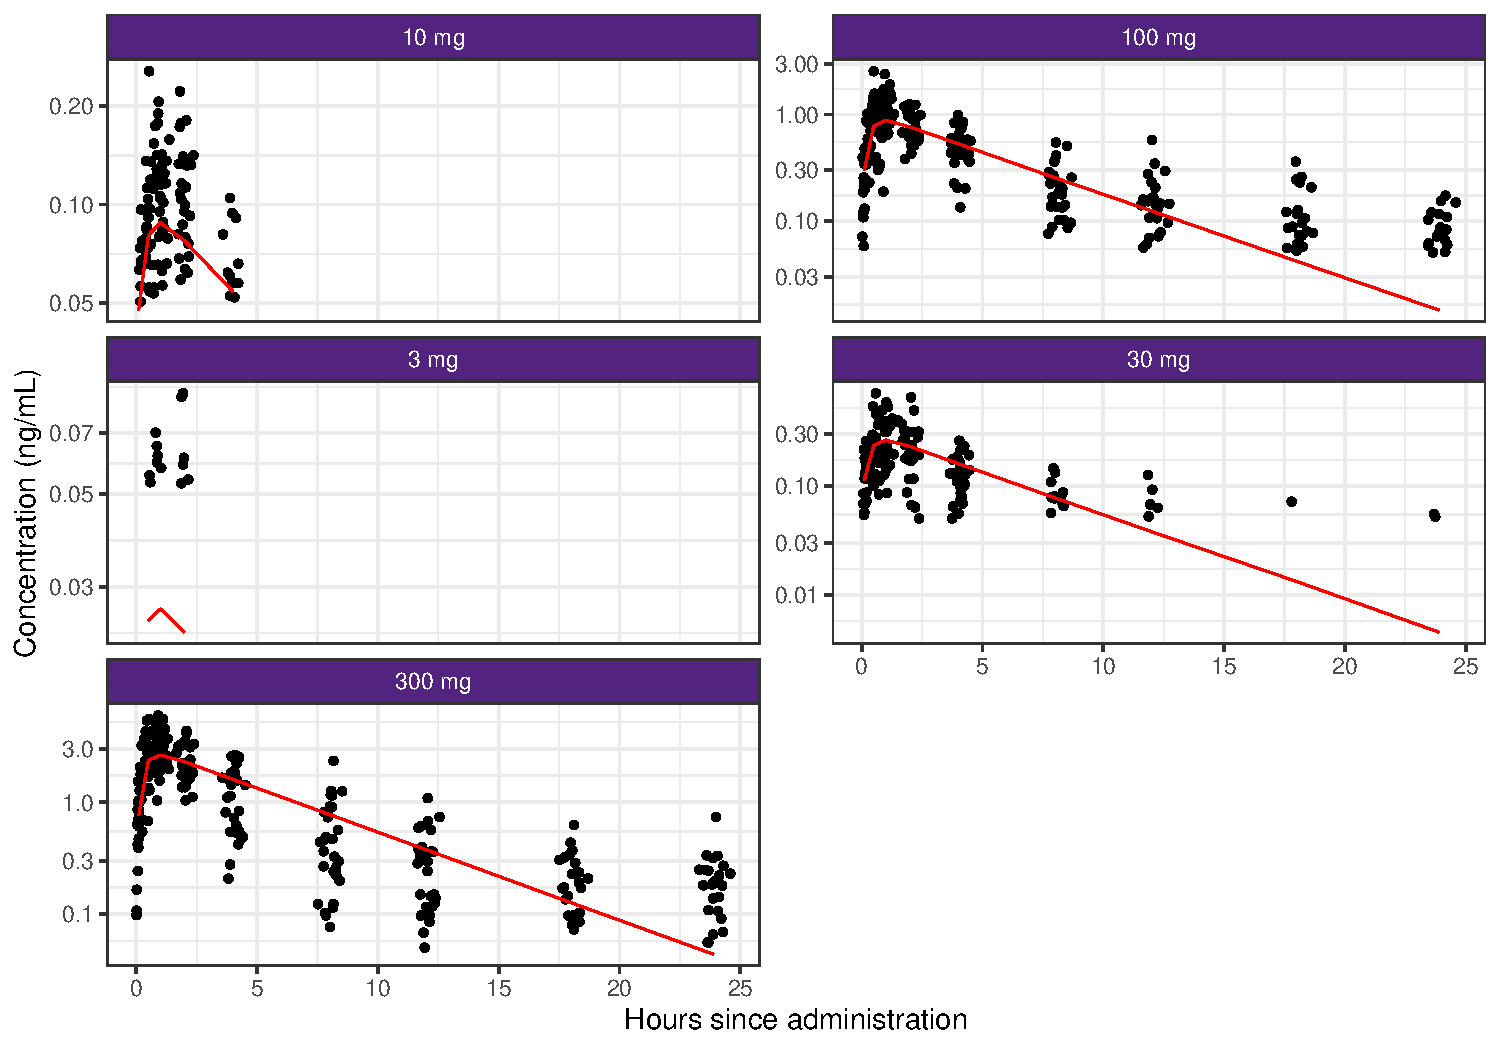
\includegraphics[width=1.05\linewidth]{plots/aplot-plot-1} \end{center}
\end{column}
\end{columns}

\end{frame}

\begin{frame}[fragile]{Recover discarded rows}
\protect\hypertarget{recover-discarded-rows}{}

\begin{columns}[T]
\begin{column}{0.45\textwidth}
\footnotesize

\begin{Shaded}
\begin{Highlighting}[]
\NormalTok{res2 <-}\StringTok{ }\KeywordTok{NMscanData}\NormalTok{(file1.lst,}
                   \DataTypeTok{merge.by.row=}\OtherTok{TRUE}\NormalTok{,}\DataTypeTok{recover.rows=}\OtherTok{TRUE}\NormalTok{)}
\end{Highlighting}
\end{Shaded}

\begin{verbatim}
## Model:  xgxr003 
## 
## Used tables, contents shown as used/total:
##                  file      rows columns     IDs
##       xgxr003_res.txt   905/905     7/7 150/150
##  xgxr003_res_vols.txt   905/905     3/7 150/150
##    xgxr003_res_fo.txt   150/150     1/2 150/150
##     xgxr1.csv (input) 1502/1502   21/24 150/150
##              (result)      1502    32+2     150
## 
## Input and output data merged by: ROW 
## 
## Distribution of rows on event types in returned data:
##  EVID CMT input-only output result
##     0   1          2      0      2
##     0   2        595    755   1350
##     1   1          0    150    150
##   All All        597    905   1502
\end{verbatim}

\begin{itemize}
\tightlist
\item
  No information is carried from output tables to recovered input data
  rows. For instance, it could make sense to merge back unique values
  within subjects (like subject level parameter estimates). Such
  ``back-filling'' must be done manually.
\end{itemize}
\end{column}

\begin{column}{0.55\textwidth}
\begin{verbatim}
## Warning: Removed 7 row(s) containing missing values
## (geom_path).
\end{verbatim}

\begin{center}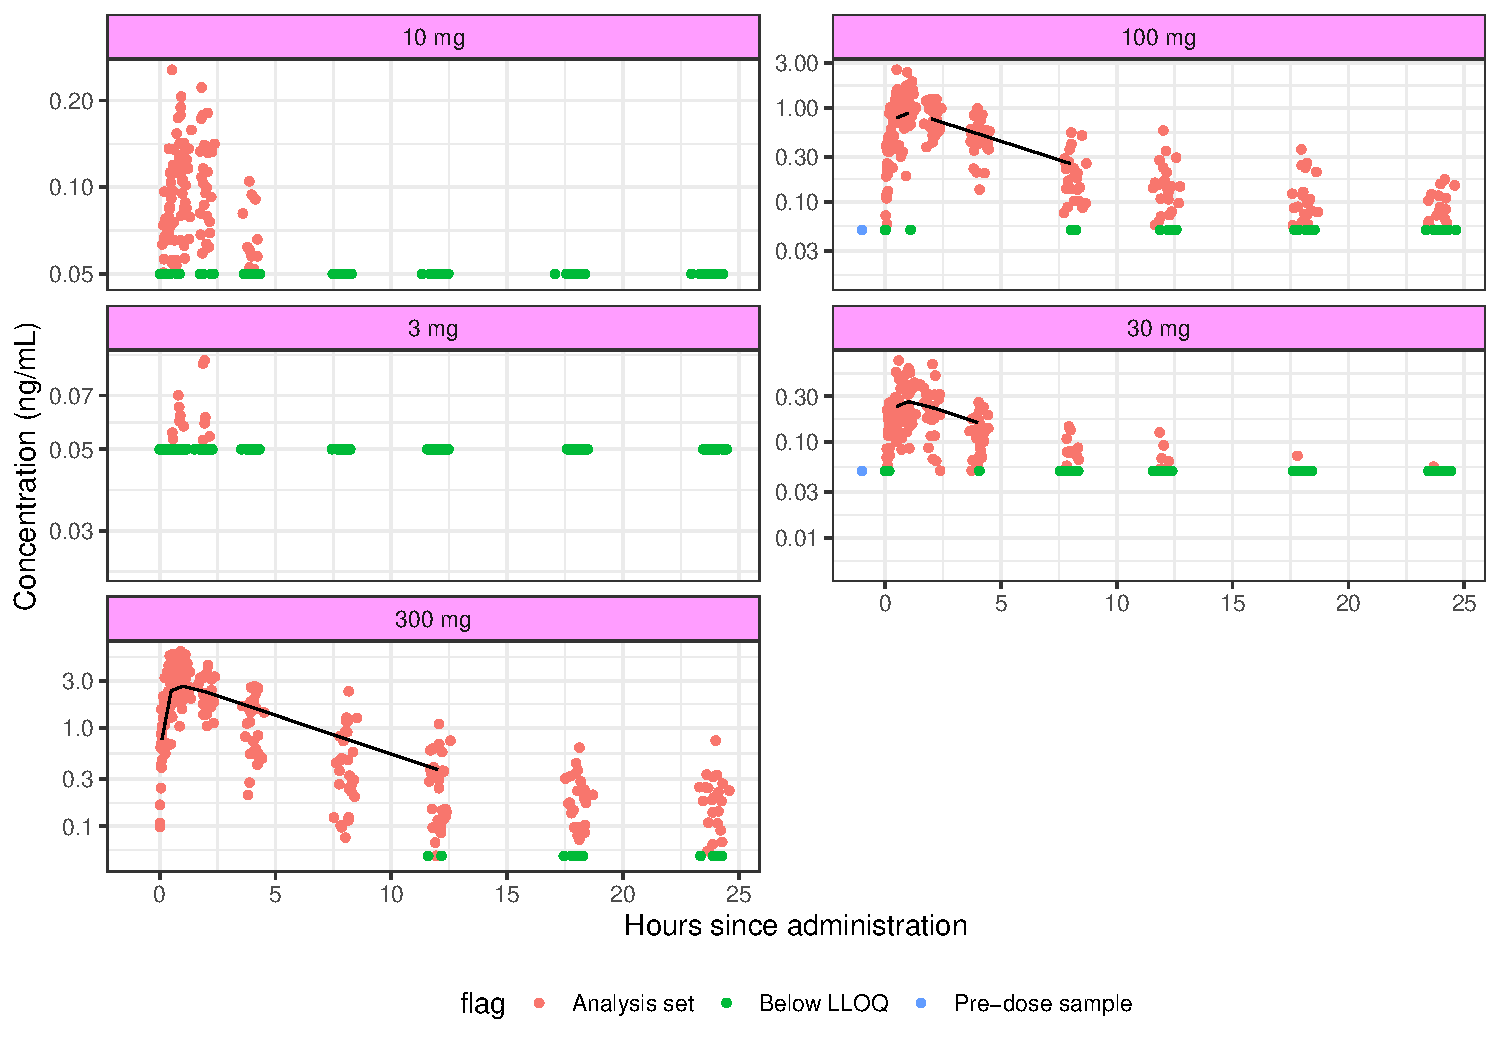
\includegraphics[width=1.05\linewidth]{plots/unnamed-chunk-34-1} \end{center}
\end{column}
\end{columns}

\end{frame}

\begin{frame}[fragile]{Compare models using \texttt{NMscanMultiple}}
\protect\hypertarget{compare-models-using-nmscanmultiple}{}

A wrapper of \texttt{NMscanData} that reads and stacks multiple models.

\begin{columns}[T]
\begin{column}{0.45\textwidth}
\footnotesize

\begin{itemize}
\tightlist
\item
  A simple example comparing a single-compartment and a two-compartment
  model.
\end{itemize}

\begin{Shaded}
\begin{Highlighting}[]
\NormalTok{models <-}\StringTok{ }\KeywordTok{file.nm}\NormalTok{(}\KeywordTok{c}\NormalTok{(}\StringTok{"xgxr001.lst"}\NormalTok{,}\StringTok{"xgxr014.lst"}\NormalTok{))}

\NormalTok{res.mult <-}\StringTok{ }\KeywordTok{NMscanMultiple}\NormalTok{(}\DataTypeTok{files=}\NormalTok{models,}\DataTypeTok{quiet=}\NormalTok{T)}
\end{Highlighting}
\end{Shaded}

\begin{verbatim}
## 
## Overview of model scanning results:
##                                                                  lst
## 1: /data/home/philipde/wdirs/NMdata/inst/examples/nonmem/xgxr001.lst
## 2: /data/home/philipde/wdirs/NMdata/inst/examples/nonmem/xgxr014.lst
##    nrows ncols success warning
## 1:   905    40    TRUE   FALSE
## 2:   905    36    TRUE   FALSE
\end{verbatim}

\begin{Shaded}
\begin{Highlighting}[]
\CommentTok{## Deriving geometric mean PRED vs time for each}
\CommentTok{## model and treatment}
\NormalTok{res.mult[EVID}\OperatorTok{==}\DecValTok{0}\OperatorTok{&}\NormalTok{nmout}\OperatorTok{==}\OtherTok{TRUE}\NormalTok{,}
\NormalTok{         gmPRED}\OperatorTok{:}\ErrorTok{=}\KeywordTok{exp}\NormalTok{(}\KeywordTok{mean}\NormalTok{(}\KeywordTok{log}\NormalTok{(PRED))),}
\NormalTok{         by=.(model,trtact,NOMTIME)]}
\end{Highlighting}
\end{Shaded}

\begin{itemize}
\tightlist
\item
  \texttt{NMscanMultiple} can search for models by matching file names
  to a regular expression, similarly to \texttt{NMwriteSection}.
\end{itemize}
\end{column}

\begin{column}{0.55\textwidth}
\normalsize

\begin{center}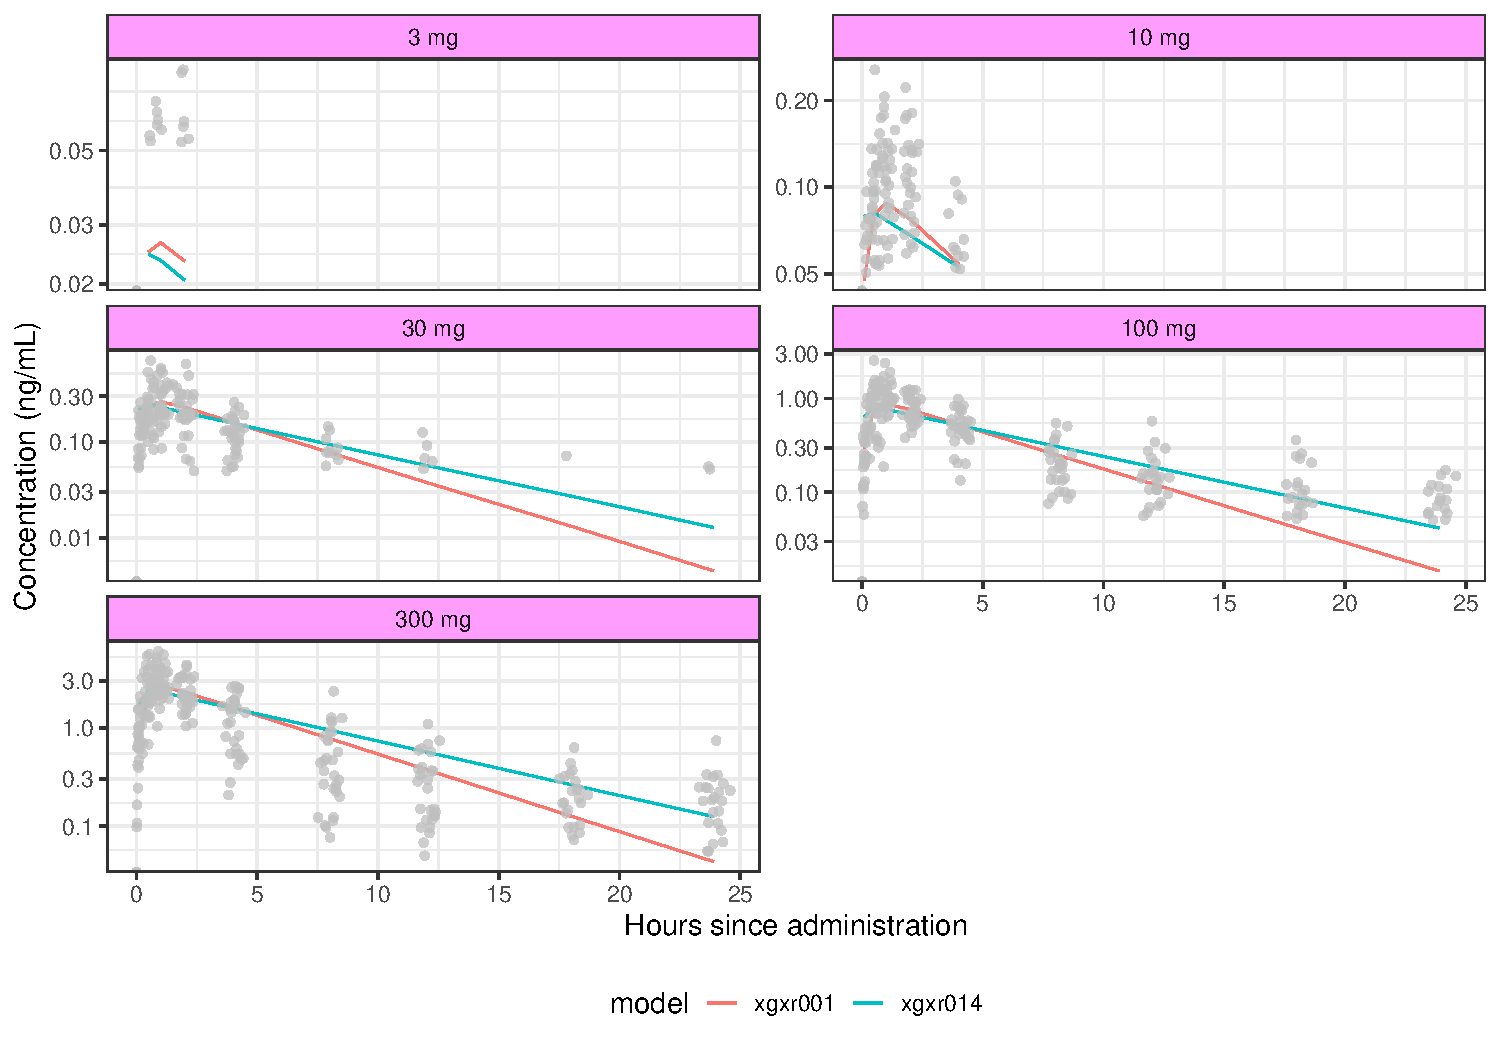
\includegraphics{plots/comparemodels-plot-1} \end{center}
\end{column}
\end{columns}

\end{frame}

\begin{frame}[fragile]{Preserve all input data properties}
\protect\hypertarget{preserve-all-input-data-properties}{}

\begin{columns}[T]
\begin{column}{0.48\textwidth}
By default, \texttt{NMscanData} will look for an rds file next to the
csv file (same file name, only extension .rds different).

\begin{itemize}
\item
  If this is found, it will be read, providing an enriched
  (e.g.~conserving factor levels and any other information).
\item
  There are no checks of consistency of \texttt{rds} file against
  delimited file read by \texttt{Nonmem}.
\item
  I am interested in ideas on how to do this. If we can avoid reading
  the csv file, it would be highly prefered.
\item
  You get the rds automatically if using \texttt{NMwriteData}.
\item
  Disable looking for the rds by argument \texttt{use.rds=FALSE}.
\item
  Default value of \texttt{use.rds} can be modified with
  \texttt{NMdataConf}.
\end{itemize}
\end{column}

\begin{column}{0.48\textwidth}
The plots are correctly ordered by doses - because they are ordered by
factor levels as in \texttt{rds} input data.

\footnotesize

\begin{Shaded}
\begin{Highlighting}[]
\NormalTok{lst <-}\StringTok{ }\KeywordTok{system.file}\NormalTok{(}\StringTok{"examples/nonmem/xgxr014.lst"}\NormalTok{,}
                   \DataTypeTok{package=}\StringTok{"NMdata"}\NormalTok{)}
\NormalTok{res14 <-}\StringTok{ }\KeywordTok{NMscanData}\NormalTok{(lst,}\DataTypeTok{quiet=}\OtherTok{TRUE}\NormalTok{)}
\end{Highlighting}
\end{Shaded}

\begin{center}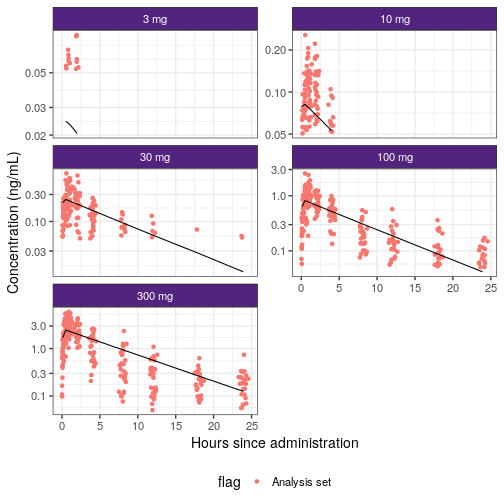
\includegraphics[width=1.05\linewidth]{plots/unnamed-chunk-37-1} \end{center}
\end{column}
\end{columns}

\normalsize

\end{frame}

\begin{frame}[fragile]{The NMdata class}
\protect\hypertarget{the-nmdata-class}{}

\begin{columns}[T]
\begin{column}{0.48\textwidth}
Most important message: an \texttt{NMdata} object can be used as if it
weren't.

Methods defined for \texttt{NMdata}:

\begin{itemize}
\tightlist
\item
  \texttt{summary}: The information that is written to the console if
  \texttt{quiet=FALSE}.
\end{itemize}

Simple other methods like \texttt{rbind} and similar are defined by
dropping the \texttt{NMdata} class and then perform the operation.

\begin{itemize}
\tightlist
\item
  \texttt{NMinfo} lists metadata from \texttt{NMdata} objects and only
  works on \texttt{NMdata} objects. Components in metadata are (as
  available):
\item
  \texttt{NMinfo(res1,"details")}: How was the data read and combined?
\item
  \texttt{NMinfo(res1,"dataCreate")}: Meta data found attached to the
  input data file.
\item
  \texttt{NMinfo(res1,"input.colnames")}: The translation table of input
  column names from input to output
\item
  \texttt{NMinfo(res1,"input.filters")}: The ``filters'' (IGNORE/ACCEPT)
  from Nonmem and how they are applied in R.
\item
  \texttt{NMinfo(res1,"tables")}: What tables were read and how?
\item
  \texttt{NMinfo(res1,"columns")}: What columns were read from what
  tables?
\end{itemize}
\end{column}

\begin{column}{0.48\textwidth}
\tiny

\begin{Shaded}
\begin{Highlighting}[]
\KeywordTok{class}\NormalTok{(res1)}
\end{Highlighting}
\end{Shaded}

\begin{verbatim}
## [1] "NMdata"     "data.table" "data.frame"
\end{verbatim}

\begin{Shaded}
\begin{Highlighting}[]
\KeywordTok{NMinfo}\NormalTok{(res1,}\StringTok{"details"}\NormalTok{)}
\end{Highlighting}
\end{Shaded}

\begin{verbatim}
## $model
## [1] "xgxr003"
## 
## $call
## [1] "NMscanData(file1.lst, merge.by.row = TRUE, as.fun = \"data.table\", "
## [2] "    quiet = TRUE)"                                                   
## 
## $time.NMscanData
## [1] "2022-06-30 13:44:29 EDT"
## 
## $file.lst
## [1] "/data/home/philipde/wdirs/NMdata/inst/examples/nonmem/xgxr003.lst"
## 
## $file.mod
## [1] "/data/home/philipde/wdirs/NMdata/inst/examples/nonmem/xgxr003.mod"
## 
## $time.ok
## [1] "Not checked"
## 
## $dir.data
## NULL
## 
## $input.used
## [1] TRUE
## 
## $rows.recovered
## [1] FALSE
## 
## $merge.by.row
## [1] TRUE
## 
## $col.row
## [1] "ROW"
## 
## $file.input
## [1] "/data/home/philipde/wdirs/NMdata/inst/examples/nonmem/../data/xgxr1.csv"
## 
## $logtime.lst
## [1] NA
## 
## $mtime.lst
## [1] "2022-05-17 15:28:08 EDT"
## 
## $method.time.lst
## [1] NA
## 
## $mtime.mod
## [1] "2022-05-17 15:28:08 EDT"
## 
## $mtime.input
## [1] "2022-05-14 23:22:02 EDT"
## 
## $logtime.input
## [1] NA
## 
## $method.time.inp
## [1] NA
\end{verbatim}
\end{column}
\end{columns}

\end{frame}

\begin{frame}[fragile]{The NMdata class}
\protect\hypertarget{the-nmdata-class-1}{}

\framesubtitle{What data was read?}

\begin{columns}[T]
\begin{column}{0.48\textwidth}
\begin{block}{Table-specific information}

\scriptsize

\begin{Shaded}
\begin{Highlighting}[]
\KeywordTok{NMinfo}\NormalTok{(res1,}\StringTok{"tables"}\NormalTok{)}
\end{Highlighting}
\end{Shaded}

\begin{verbatim}
##    source                 name nrow ncol nid level
## 1: output      xgxr003_res.txt  905    7  NA   row
## 2: output xgxr003_res_vols.txt  905    7 150   row
## 3: output   xgxr003_res_fo.txt  150    2 150    id
## 4:  input            xgxr1.csv 1502   24 150  <NA>
##        scope has.col.row has.col.id full.length filetype
## 1:       all        TRUE      FALSE        TRUE   output
## 2:       all       FALSE       TRUE        TRUE   output
## 3: firstonly       FALSE       TRUE       FALSE   output
## 4:      <NA>        TRUE       TRUE          NA     text
##      format          file.mtime
## 1:          2022-05-17 15:28:08
## 2:   tF13.4 2022-05-17 15:28:08
## 3: ,1PE15.8 2022-05-17 15:28:08
## 4:     <NA> 2022-05-14 23:22:02
##                                                                          file
## 1:      /data/home/philipde/wdirs/NMdata/inst/examples/nonmem/xgxr003_res.txt
## 2: /data/home/philipde/wdirs/NMdata/inst/examples/nonmem/xgxr003_res_vols.txt
## 3:   /data/home/philipde/wdirs/NMdata/inst/examples/nonmem/xgxr003_res_fo.txt
## 4:    /data/home/philipde/wdirs/NMdata/inst/examples/nonmem/../data/xgxr1.csv
##    noheader file.logtime
## 1:    FALSE           NA
## 2:    FALSE           NA
## 3:    FALSE           NA
## 4:       NA           NA
\end{verbatim}

\end{block}
\end{column}

\begin{column}{0.48\textwidth}
\begin{block}{Column-specific information}

(The \texttt{nrows} and \texttt{topn} arguments are arguments to
\texttt{print.data.table} to get a top and bottom snip of the table.)
\scriptsize

\begin{Shaded}
\begin{Highlighting}[]
\KeywordTok{print}\NormalTok{(}\KeywordTok{NMinfo}\NormalTok{(res1,}\StringTok{"columns"}\NormalTok{),}\DataTypeTok{nrows=}\DecValTok{20}\NormalTok{,}\DataTypeTok{topn=}\DecValTok{10}\NormalTok{)}
\end{Highlighting}
\end{Shaded}

\begin{verbatim}
##     variable                 file     source level COLNUM
##  1:      ROW      xgxr003_res.txt     output   row      1
##  2:       ID xgxr003_res_vols.txt     output   row      2
##  3:  NOMTIME            xgxr1.csv      input   row      3
##  4:     TIME            xgxr1.csv      input   row      4
##  5:     EVID            xgxr1.csv      input   row      5
##  6:      CMT            xgxr1.csv      input   row      6
##  7:      AMT            xgxr1.csv      input   row      7
##  8:       DV      xgxr003_res.txt     output   row      8
##  9:     FLAG            xgxr1.csv      input   row      9
## 10:    STUDY            xgxr1.csv      input   row     10
## ---                                                      
## 33:    model                 <NA> NMscanData model     33
## 34:    nmout                 <NA> NMscanData   row     34
## 35:       DV xgxr003_res_vols.txt     output   row     NA
## 36:     PRED xgxr003_res_vols.txt     output   row     NA
## 37:      RES xgxr003_res_vols.txt     output   row     NA
## 38:     WRES xgxr003_res_vols.txt     output   row     NA
## 39:      ROW            xgxr1.csv      input   row     NA
## 40:       ID            xgxr1.csv      input   row     NA
## 41:       DV            xgxr1.csv      input   row     NA
## 42:       ID   xgxr003_res_fo.txt     output    id     NA
\end{verbatim}

\end{block}
\end{column}
\end{columns}

\end{frame}

\begin{frame}[fragile]{What to do when Nonmem results seem meaningless?}
\protect\hypertarget{what-to-do-when-nonmem-results-seem-meaningless}{}

\framesubtitle{Check of usual suspect: DATA}

\begin{columns}[T]
\begin{column}{0.48\textwidth}
\begin{itemize}
\tightlist
\item
  \texttt{NMcheckColnames} lists column names
\item
  As in input data set
\item
  As in Nonmem \texttt{\$DATA}
\item
  As inferred by \texttt{NMscanInput} (and \texttt{NMscanData})
\item
  This will help you easily check if \texttt{\$DATA} matches the input
  data file.
\item
  This is a new function that will be available in the next
  \texttt{NMdata} release
\item
  A more advanced idea is some automated guessing if mistakes were made.
  This is currently not on the todo list
\end{itemize}
\end{column}

\begin{column}{0.48\textwidth}
In this case, input column names are aligned with \texttt{\$DATA}
\footnotesize

\begin{Shaded}
\begin{Highlighting}[]
\KeywordTok{NMcheckColnames}\NormalTok{(lst)}
\end{Highlighting}
\end{Shaded}

\begin{verbatim}
## Read rds input data file:
## /data/home/philipde/wdirs/NMdata/inst/examples/nonmem/../data/xgxr2.rds.
\end{verbatim}

\begin{verbatim}
##     datafile    INPUT   nonmem   result compare
##  1:      ROW      ROW      ROW      ROW      OK
##  2:       ID       ID       ID       ID      OK
##  3:  NOMTIME  NOMTIME  NOMTIME  NOMTIME      OK
##  4:     TIME     TIME     TIME     TIME      OK
##  5:     EVID     EVID     EVID     EVID      OK
##  6:      CMT      CMT      CMT      CMT      OK
##  7:      AMT      AMT      AMT      AMT      OK
##  8:       DV       DV       DV       DV      OK
##  9:     FLAG     FLAG     FLAG     FLAG      OK
## 10:    STUDY    STUDY    STUDY    STUDY      OK
## 11:      BLQ      BLQ      BLQ      BLQ      OK
## 12:    CYCLE    CYCLE    CYCLE    CYCLE      OK
## 13:     DOSE     DOSE     DOSE     DOSE      OK
## 14:     PART     PART     PART     PART      OK
## 15:  PROFDAY  PROFDAY  PROFDAY  PROFDAY      OK
## 16: PROFTIME PROFTIME PROFTIME PROFTIME      OK
## 17:  WEIGHTB  WEIGHTB  WEIGHTB  WEIGHTB      OK
## 18:     eff0     eff0     eff0     eff0      OK
## 19:   EVENTU     <NA>     <NA>   EVENTU    <NA>
## 20:     NAME     <NA>     <NA>     NAME    <NA>
## 21: TIMEUNIT     <NA>     <NA> TIMEUNIT    <NA>
## 22:   TRTACT     <NA>     <NA>   TRTACT    <NA>
## 23:     flag     <NA>     <NA>     flag    <NA>
## 24:   trtact     <NA>     <NA>   trtact    <NA>
##     datafile    INPUT   nonmem   result compare
\end{verbatim}

\normalsize
\end{column}
\end{columns}

\end{frame}

\begin{frame}[fragile]{What should I do for my models to be compatible
with \texttt{NMscanData}?}
\protect\hypertarget{what-should-i-do-for-my-models-to-be-compatible-with-nmscandata}{}

\begin{itemize}
\item
  The answer to this should be as close to ``nothing'' as possible -
  that's more or less the aim of the function.
\item
  (As always) you just have to make sure that the information that you
  need is present in input data and output data.
\item
  No need to output information that is unchanged from input, but make
  sure to output what you need (like \texttt{IPRED}, \texttt{CWRES},
  \texttt{CL}, \texttt{ETA1} etc which cannot be found in input). Always
  output the row identifier!
\item
  Some of these values can be found from other files generated by
  \texttt{Nonmem} but notice: \texttt{NMscanData} only uses input and
  output data.
\item
  Including a unique row identifier in both input and output data is the
  most robust way to combine the tables.
\item
  Everything will most likely work even if you don't
\item
  I would not take ``most likely'' when robustness is available.
\item
  In \texttt{firstonly} tables, include the subject ID or the row
  identifier.
\end{itemize}

\end{frame}

\begin{frame}[fragile]{\texttt{NMscanData} limitations}
\protect\hypertarget{nmscandata-limitations}{}

The most important limitation to have in mind is not related to
\texttt{NMscanData} iteself

\begin{itemize}
\tightlist
\item
  If merging with input data, the input data must be available as was
  when the model was run.
\item
  Option 1: ``Freeze'' model runs together with data.
  \texttt{NMfreezeModels} does that and will be included in
  \texttt{NMdata} after a little more testing.
\item
  Option 2 (platform-dependent): \texttt{Nonmem} can be run in a wrapper
  script that either copies the input data, or runs \texttt{NMscanData}
  and saves the output in a compressed file format (like \texttt{rds}).
\end{itemize}

Even if limitations of \texttt{NMscanData} may be several, they are all
rare. There is a very good chance you will never run into any of them.

\begin{itemize}
\item
  Not all data filter statements implemented. Nested \texttt{ACCEPT} and
  \texttt{IGNORE} statements are not supported at this point. The
  resulting number of rows after applying filters is checked against
  row-level output table dimensions (if any available).
\item
  Disjoint rows with common \texttt{ID} values are currently not
  supported together with \texttt{firstonly} or \texttt{lastonly}
  tables. This is on the todo list.
\item
  The \texttt{RECORDS} and \texttt{NULL} options in \texttt{\$DATA} are
  not implemented. If using \texttt{RECORDS}, please use the
  \texttt{col.row} option to merge by a unique row identifier.
\item
  Character time variables not interpreted. If you need this, we can
  implement it relatively easily.
\item
  Only output tables returning either all rows or one row per subject
  can be merged with input. Tables written with options like
  \texttt{FIRSTLASTONLY} (two rows per subject) and \texttt{OBSONLY} are
  disregarded with a warning (you can read them with
  \texttt{NMscanTables}). \texttt{LASTONLY} is treated like
  \texttt{FIRSTONLY}, i.e.~as ID-level information if not available
  elsewhere.
\end{itemize}

\end{frame}

\begin{frame}[fragile]{Data read building blocks}
\protect\hypertarget{data-read-building-blocks}{}

\texttt{NMscanData} uses a few simpler functions to read all the data it
can find. These functions may be useful when you don't want the full
automatic package provided by \texttt{NMscanData}.

\begin{itemize}
\tightlist
\item
  \texttt{NMreadTab}

  \begin{itemize}
  \tightlist
  \item
    Fast read and format output tables from Nonmem
  \item
    Handles the ``\texttt{TABLE\ NO.}'' counter
  \item
    If you simulate a large number of subjects in Nonmem and get a large
    (gigabytes) output data file, this will be extremely fast compared
    to almost anything else.
  \end{itemize}
\item
  \texttt{NMscanTables} (uses \texttt{NMreadTab})

  \begin{itemize}
  \tightlist
  \item
    Given a control stream or list file, read all output tables
  \end{itemize}
\item
  \texttt{NMreadCsv}

  \begin{itemize}
  \tightlist
  \item
    Fast read delimited (input data) files
  \end{itemize}
\item
  \texttt{NMscanInput} (uses \texttt{NMreadCSV})

  \begin{itemize}
  \tightlist
  \item
    Given a control stream or list file, read input data.
  \item
    Optionally reads and applies Nonmem ignore/accept statements
  \item
    Optionally translates column names according to names used in Nonmem
  \end{itemize}
\end{itemize}

\end{frame}

\hypertarget{configuration-of-nmdata-defaults}{%
\section{Configuration of NMdata
defaults}\label{configuration-of-nmdata-defaults}}

\begin{frame}[fragile]{NMdataConf}
\protect\hypertarget{nmdataconf}{}

\framesubtitle{Tailor `NMdata` default behavior to your setup and preferences}

\begin{columns}[T]
\begin{column}{0.48\textwidth}
\begin{itemize}
\item
  \texttt{NMdataConf} supports changing many default argument values,
  simplifying coding.
\item
  Notice, values are reset when \texttt{library(NMdata)} or
  \texttt{NMdataConf(reset=TRUE)} are called.
\item
  See all currently used values by \texttt{NMdataConf()}.
\end{itemize}
\end{column}

\begin{column}{0.48\textwidth}
My initialization of scripts often contain this:

\begin{Shaded}
\begin{Highlighting}[]
\KeywordTok{library}\NormalTok{(NMdata)}
\KeywordTok{NMdataConf}\NormalTok{(}\DataTypeTok{as.fun=}\StringTok{"data.table"}
\CommentTok{### this is the default value}
\NormalTok{          ,}\DataTypeTok{col.row=}\StringTok{"ROW"}
\CommentTok{### Recommended but _right now_ not default}
\NormalTok{          ,}\DataTypeTok{merge.by.row=}\OtherTok{TRUE}
\CommentTok{### You can switch this when script is final}
\NormalTok{          ,}\DataTypeTok{quiet=}\OtherTok{FALSE}\NormalTok{)}
\end{Highlighting}
\end{Shaded}
\end{column}
\end{columns}

Other commonly used settings in \texttt{NMdataConf} are

\begin{itemize}
\tightlist
\item
  \texttt{as.fun}: a function to apply to all objects before returning
  them from \texttt{NMdata} functions. If you use
  \texttt{dplyr/tidyverse}, do (notice, no quotes!):
\end{itemize}

\begin{Shaded}
\begin{Highlighting}[]
\KeywordTok{library}\NormalTok{(tibble)}
\KeywordTok{NMdataConf}\NormalTok{(}\DataTypeTok{as.fun=}\NormalTok{tibble}\OperatorTok{::}\NormalTok{as_tibble)}
\end{Highlighting}
\end{Shaded}

\begin{itemize}
\item
  \texttt{use.input}: Should \texttt{NMscanData} combine (output data)
  with input data? (default \texttt{TRUE})
\item
  \texttt{recover.rows}: Should \texttt{NMscanData} Include rows not
  processed by Nonmem? (default \texttt{FALSE}).
\item
  \texttt{file.mod}: A function that translates the list file path to
  the input control stream file path. Default is to replace extension
  with \texttt{.mod}.
\item
  \texttt{check.time}: Default is \texttt{TRUE}, meaning that output
  (list file and tables) are expected to newer than input (control
  stream and input data). If say you copy files between systems, this
  check may not make sense.
\end{itemize}

\end{frame}

\begin{frame}[fragile]{Why does \texttt{NMdata} not use
\texttt{options()}?}
\protect\hypertarget{why-does-nmdata-not-use-options}{}

\texttt{R} has a system for handling settings. \texttt{NMdata} does not
use that.

\begin{itemize}
\tightlist
\item
  Main reason: \texttt{NMdataConf} can check both setting/argument names
  and values for consistency.
\end{itemize}

\begin{Shaded}
\begin{Highlighting}[]
\KeywordTok{try}\NormalTok{(}\KeywordTok{NMdataConf}\NormalTok{(}\DataTypeTok{asfun=}\NormalTok{tibble}\OperatorTok{::}\NormalTok{as_tibble))}
\end{Highlighting}
\end{Shaded}

\begin{verbatim}
## Error : Option not found
\end{verbatim}

\begin{Shaded}
\begin{Highlighting}[]
\KeywordTok{try}\NormalTok{(}\KeywordTok{NMdataConf}\NormalTok{(}\DataTypeTok{use.input=}\StringTok{"FALSE"}\NormalTok{))}
\end{Highlighting}
\end{Shaded}

\begin{verbatim}
## Error : use.input must be logical
\end{verbatim}

\begin{itemize}
\tightlist
\item
  A few extra features are available with \texttt{NMdataConf}:
\item
  Reset all settings: \texttt{NMdataConf(reset=TRUE)}
\item
  Reset individual settings:
  \texttt{NMdataConf(use.input=NULL,\ as.fun=NULL)}
\item
  Retrieve all current settings: \texttt{NMdataConf()}
\end{itemize}

\end{frame}

\begin{frame}[fragile]{How is \texttt{NMdata} qualified?}
\protect\hypertarget{how-is-nmdata-qualified}{}

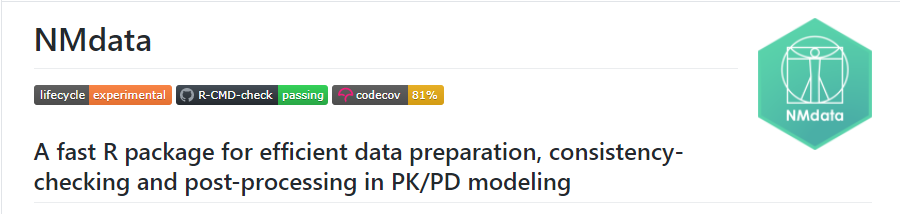
\includegraphics[width=.8\textwidth]{badges_snip_210623}

\begin{itemize}
\item
  \texttt{NMdata} contains very little calculations (only exception may
  be \texttt{flagsAssign}/\texttt{flagsCount})
\item
  Historic bugs have mostly resulted in uninformative errors due to
  e.g.~failure in processing text. Never a wrong data set.
\item
  \texttt{NMdata} includes 190 ``unit tests'' where results of function
  calls with different datasets and arguments are compared to expected
  results
\item
  Tests are consistently run before any release of the package
\item
  The tests are crucial in making sure that fixing one bug or
  introducing a new feature does not introduce new bugs
\item
  The testing approach is as recommended in ``R packages'' by Hadley
  Wickham and Jennifer Bryan \url{https://r-pkgs.org/tests.html}.
\item
  If you have a specific example you want to make sure is tested in the
  package, we will include the test in the package
\end{itemize}

\end{frame}

\hypertarget{next-steps-for-nmdata}{%
\section{\texorpdfstring{Next steps for
\texttt{NMdata}}{Next steps for NMdata}}\label{next-steps-for-nmdata}}

\begin{frame}[fragile]{Next steps for \texttt{NMdata}}
\protect\hypertarget{next-steps-for-nmdata-1}{}

\begin{itemize}
\item
  The following would be great help in making \texttt{NMdata} more
  accessible and useful
\item
  Testing - please use the package and provide feedback
\item
  Review of documentation, vignettes, and descriptions/explanations on
  website
\item
  Graphical representations and illustrations.
\item
  A tidyverse workflow for a new vignette
\item
  If you have ideas you want to contribute, let's discuss!
\item
  Additional features
\item
  Functions to generate dosing regimens for simulations and nominal-time
  datasets
\item
  Functions for easy documentation of column contents (description,
  units, 1:1 relationships between character and numeric columns)
\item
  \texttt{NMfreezeModels}: Save Nonmem models with input data and all
  results to ensure reproducibility of output 
\end{itemize}

\end{frame}

\hypertarget{summary}{%
\section{Summary}\label{summary}}

\begin{columns}[T]
\begin{column}{0.48\textwidth}
Data creation

\begin{itemize}
\tightlist
\item
  \texttt{renameByContents}
\item
  \texttt{compareCols}
\item
  \texttt{mergeCheck}
\item
  \texttt{flagsAssign}/\texttt{flagsCount}
\item
  \texttt{NMorderColumns}
\item
  (\texttt{NMcheckData})
\item
  \texttt{NMwriteData}
\item
  \texttt{NMstamp}/\texttt{NMinfo}
\end{itemize}

Read/write Nonmem control streams

\begin{itemize}
\tightlist
\item
  \texttt{NMreadSection}/\texttt{NMwriteSection}
\end{itemize}
\end{column}

\begin{column}{0.48\textwidth}
Retrieve data from Nonmem runs

\begin{itemize}
\tightlist
\item
  \texttt{NMscanData}
\item
  \texttt{NMscanMultiple}
\item
  \texttt{summary}, \texttt{NMinfo}
\item
  \texttt{NMscanInput}, \texttt{NMreadCsv}
\item
  \texttt{NMscanTables}, \texttt{NMreadTab}
\item
  \texttt{NMcheckColnames}
\end{itemize}

Adjust behavior to your preferences

\begin{itemize}
\tightlist
\item
  \texttt{NMdataConf}
\end{itemize}

Other

\begin{itemize}
\tightlist
\item
  (\texttt{NMfreezeModels})
\end{itemize}
\end{column}
\end{columns}

\hypertarget{nmdata-functions-under-development}{%
\section{\texorpdfstring{\texttt{NMdata} functions under
development}{NMdata functions under development}}\label{nmdata-functions-under-development}}

\begin{frame}[fragile]{NMfreezeModels}
\protect\hypertarget{nmfreezemodels}{}

\begin{columns}[T]
\begin{column}{0.85\textwidth}
In order to ensure reproducibility, any output has to be produced based
on arvhived/frozen Nonmem models.
\end{column}

\begin{column}{0.15\textwidth}

\includegraphics[width=.5in]{figures/worksign.png}
\end{column}
\end{columns}

The components that need to be ``frozen'' are

\begin{itemize}
\tightlist
\item
  Nonmem control streams
\item
  input data
\item
  estimation results (output tables, .lst, .ext etc.)
\item
  simulation code (say mrgsolve scripts)
\item
  ?
\end{itemize}

\texttt{NMfreezeModels} does freeze

\begin{itemize}
\tightlist
\item
  input control streams
\item
  input data
\item
  all output tables
\item
  all nonmem results files
\end{itemize}

Limitations

\begin{itemize}
\tightlist
\item
  NMfreezeModels does not provide a solution for the simulation code at
  this point. I am very interested in how we can do this.
\item
  Only supports collections of models with one common input dataset
\item
  The permissions of the frozen folder should be read-only. However,
  that means that once the freeze it's done, you can no longer add code
  or descriptions. It all has to be handled in the freeze procedure.
\end{itemize}

\end{frame}

\begin{frame}{Safe model reader}
\protect\hypertarget{safe-model-reader}{}

\begin{columns}[T]
\begin{column}{0.85\textwidth}
\begin{itemize}
\item
  A function to read frozen Nonmem results and mrgsolve code to ensure
  that the right simulation model and parameter values are used
\item
  Obviously, this is closely related to the way mrgsolve code is frozen
  together with nonmem code.
\end{itemize}
\end{column}

\begin{column}{0.15\textwidth}

\includegraphics[width=.5in]{figures/ideabulb.jpg}
\end{column}
\end{columns}

\end{frame}

\hypertarget{other-tools}{%
\section{Other tools}\label{other-tools}}

\begin{frame}[fragile]{tracee}
\protect\hypertarget{tracee}{}

\begin{itemize}
\tightlist
\item
  New package on CRAN from same author as \texttt{NMdata}
\item
  A small package focusing on making outputs (graphics) traceable back
  to code
\item
  The author has been using the code for years
\end{itemize}

\end{frame}

\begin{frame}[fragile]{\texttt{ggwrite}: Flexible saving of tracable
output}
\protect\hypertarget{ggwrite-flexible-saving-of-tracable-output}{}

Saves images in sizes made for powerpoint, including stamps (time,
source, output filename). It can save multiple plots at once as one file
(pdf) or multiple files.

\begin{columns}[T]
\begin{column}{0.48\textwidth}
\texttt{ggwrite} is a wrapper of \texttt{png} and \texttt{pdf} (and
\texttt{dev.off}) with convenience features such as

\begin{itemize}
\tightlist
\item
  Support for multiple plots at once
\item
  saved as either multiple files, named by list element names if wanted
  (or just numbered)
\item
  or a single pdf with one plot per page
\item
  Stamping with creation time, script name, and output name
\item
  ``canvas'' sizes made for powerpoint or full-screen display (see
  \texttt{?canvasSize})
\item
  Custom canvases are very simple to create
\item
  Independent \texttt{save} and \texttt{show} arguments for very simple
  conditional behavior
\item
  \texttt{save} defaults to \texttt{TRUE} if a filename is given
\item
  \texttt{show} defaults to the inverse of \texttt{save}
\end{itemize}
\end{column}

\begin{column}{0.48\textwidth}
\footnotesize

\begin{Shaded}
\begin{Highlighting}[]
\NormalTok{writeOutput <-}\StringTok{ }\OtherTok{TRUE}
\NormalTok{script <-}\StringTok{ "path/to/script.R"}
\NormalTok{p1 <-}\StringTok{ }\KeywordTok{ggplot}\NormalTok{(res1,}\KeywordTok{aes}\NormalTok{(PRED,DV,}\DataTypeTok{colour=}\NormalTok{TRTACT))}\OperatorTok{+}\KeywordTok{geom_point}\NormalTok{()}\OperatorTok{+}
\StringTok{    }\KeywordTok{geom_abline}\NormalTok{(}\DataTypeTok{slope=}\DecValTok{1}\NormalTok{)}\OperatorTok{+}
\StringTok{    }\KeywordTok{scale_x_log10}\NormalTok{()}\OperatorTok{+}\KeywordTok{scale_y_log10}\NormalTok{()}
\KeywordTok{ggwrite}\NormalTok{(p1,}\DataTypeTok{file=}\StringTok{"results/pred_dv.png"}\NormalTok{,}
        \DataTypeTok{script=}\NormalTok{script,}
        \DataTypeTok{save=}\NormalTok{writeOutput)}
\end{Highlighting}
\end{Shaded}

\begin{itemize}
\tightlist
\item
  Notice the caption with output and script file names.

  \begin{center}
  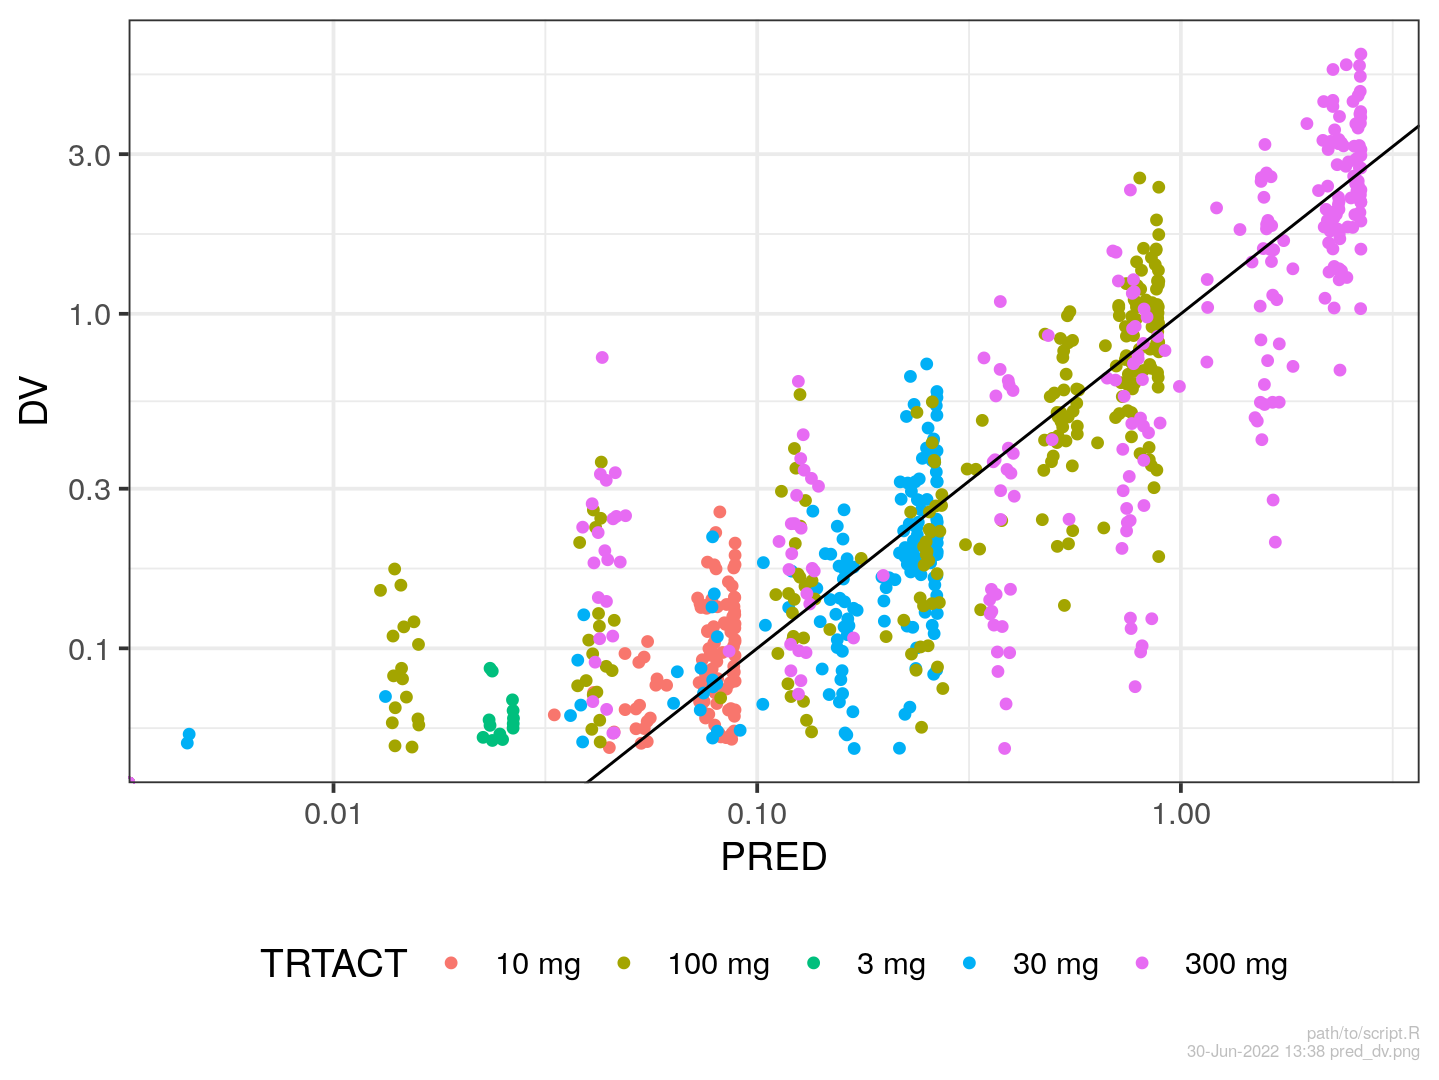
\includegraphics{results/pred_dv.png}
  \end{center}
\end{itemize}
\end{column}
\end{columns}

\end{frame}

\begin{frame}{\texttt{execSafe}: Save input data with each Nonmem run}
\protect\hypertarget{execsafe-save-input-data-with-each-nonmem-run}{}

\begin{itemize}
\tightlist
\item
  Executes Nonem from within R
\item
  Archives input data together with Nonmem run (you can tell NMdata to
  read that archive when reading your model)
\item
  Automatically generates a PNM file if you want to parallellize
\end{itemize}

\end{frame}

\end{document}
